\documentclass[11pt]{book}

%%%%%%%%%%%%%%Include Packages%%%%%%%%%%%%%%%%%%%%%%%%%%
\usepackage{xcolor}
\usepackage{mathtools}
\usepackage[a4paper, total={6in, 8in}, margin=1.25in]{geometry}
\usepackage{amsmath}
\usepackage{amssymb}
\usepackage{paralist}
\usepackage{rsfso}
\usepackage{amsthm}
\usepackage{wasysym}
\usepackage[inline]{enumitem}   
\usepackage{hyperref}
\usepackage{tocloft}
\usepackage{wrapfig}
\usepackage{titlesec}
\usepackage{colortbl}
\usepackage{stackengine} 
%%%%%%%%%%%%%%%%%%%%%%%%%%%%%%%%%%%%%%%%%%%%%%%%%%%%%%%%


%%%%%%%%%%%%%%%Chapter Setting%%%%%%%%%%%%%%%%%%%%%%%%%%
\definecolor{gray75}{gray}{0.75}
\newcommand{\hsp}{\hspace{20pt}}
\titleformat{\chapter}[hang]{\Huge\bfseries}{\thechapter\hsp\textcolor{gray75}{$\mid$}\hsp}{0pt}{\Huge\bfseries}
%%%%%%%%%%%%%%%%%%%%%%%%%%%%%%%%%%%%%%%%%%%%%%%%%%%%%%%%

%%%%%%%%%%%%%%%%%Theorem environments%%%%%%%%%%%%%%%%%%%
\newtheoremstyle{break}
  {\topsep}{\topsep}%
  {\itshape}{}%
  {\bfseries}{}%
  {\newline}{}%
\theoremstyle{break}
\theoremstyle{break}
\newtheorem{axiom}{Axiom}
\newtheorem{thm}{Theorem}[section]
\renewcommand{\thethm}{\arabic{section}.\arabic{thm}}
\newtheorem{lem}{Lemma}[thm]
\newtheorem{prop}[lem]{Proposition}
\newtheorem{corL}{Corollary}[lem]
\newtheorem{corT}[lem]{Corollary}
\newtheorem{defn}{Definition}[corL]
\newenvironment{indEnv}[1][Proof]
  {\proof[#1]\leftskip=1cm\rightskip=1cm}
  {\endproof}
%%%%%%%%%%%%%%%%%%%%%%%%%%%%%%%%%%%%%%%%%%%%%%%%%%%%%%


%%%%%%%%%%%%%%%%%%%%%%%Integral%%%%%%%%%%%%%%%%%%%%%%%
\def\upint{\mathchoice%
    {\mkern13mu\overline{\vphantom{\intop}\mkern7mu}\mkern-20mu}%
    {\mkern7mu\overline{\vphantom{\intop}\mkern7mu}\mkern-14mu}%
    {\mkern7mu\overline{\vphantom{\intop}\mkern7mu}\mkern-14mu}%
    {\mkern7mu\overline{\vphantom{\intop}\mkern7mu}\mkern-14mu}%
  \int}
\def\lowint{\mkern3mu\underline{\vphantom{\intop}\mkern7mu}\mkern-10mu\int}
%%%%%%%%%%%%%%%%%%%%%%%%%%%%%%%%%%%%%%%%%%%%%%%%%%%%%%



\newcommand{\R}{\mathbb{R}}
\newcommand{\N}{\mathbb{N}}
\newcommand{\Z}{\mathbb{Z}}
\newcommand{\Q}{\mathbb{Q}}
\newcommand{\C}{\mathbb{C}}
\newcommand{\T}{\mathcal{T}}
\newcommand{\M}{\mathcal{M}}
\newcommand{\Symm}{\text{Symm}}
\newcommand{\Alt}{\text{Alt}}
\newcommand{\Int}{\text{Int}}
\newcommand{\Bd}{\text{Bd}}
\newcommand{\Power}{\mathcal{P}}
\newcommand{\ee}[1]{\cdot 10^{#1}}
\newcommand{\spa}{\text{span}}
\newcommand{\sgn}{\text{sgn}}
\newcommand{\degr}{\text{deg}}
\newcommand{\pd}{\partial}
\newcommand{\that}[1]{\widetilde{#1}}
\newcommand{\lr}[1]{\left(#1\right)}
\newcommand{\vmat}[1]{\begin{vmatrix} #1 \end{vmatrix}}
\newcommand{\bmat}[1]{\begin{bmatrix} #1 \end{bmatrix}}
\newcommand{\pmat}[1]{\begin{pmatrix} #1 \end{pmatrix}}
\newcommand{\ket}[1]{\,| #1 \rangle}
\newcommand{\bra}[1]{\langle #1 |\,}
\newcommand{\rref}{\xrightarrow{\text{row\ reduce}}}
\newcommand{\txtarrow}[1]{\xrightarrow{\text{#1}}}
\newcommand\oast{\stackMath\mathbin{\stackinset{c}{0ex}{c}{0ex}{\ast}{\Circle}}}


\newcommand{\note}{\color{red}Note: \color{black}}
\newcommand{\remark}{\color{blue}Remark: \color{black}}
\newcommand{\example}{\color{green}Example: \color{black}}
\newcommand{\exercise}{\color{green}Exercise: \color{black}}

%%%%%%%%%%%%%%%%%%%%%%Roman Number%%%%%%%%%%%%%%%%%%%%%%%
\makeatletter
\newcommand*{\rom}[1]{\expandafter\@slowromancap\romannumeral #1@}
\makeatother
%%%%%%%%%%%%%%%%%%%%%%%%%%%%%%%%%%%%%%%%%%%%%%%%%%%%%%%%%

%%%%%%%%%%%%table of contents%%%%%%%%%%%%%%%%%%%%%%%%%%%%
\setlength{\cftchapindent}{0em}
\cftsetindents{section}{2em}{3em}

\renewcommand\cfttoctitlefont{\hfill\huge\bfseries}
\renewcommand\cftaftertoctitle{\hfill\mbox{}}

\setcounter{tocdepth}{2}
%%%%%%%%%%%%%%%%%%%%%%%%%%%%%%%%%%%%%%%%%%%%%%%%%%%%%%%%%


%%%%%%%%%%%%%%%%%%%%%Footnotes%%%%%%%%%%%%%%%%%%%%%%%%%%%
\newcommand\blfootnote[1]{%
  \begingroup
  \renewcommand\thefootnote{}\footnote{#1}%
  \addtocounter{footnote}{-1}%
  \endgroup
}
%%%%%%%%%%%%%%%%%%%%%%%%%%%%%%%%%%%%%%%%%%%%%%%%%%%%%%%%%

%%%%%%%%%%%%%%%%%%%%%Section%%%%%%%%%%%%%%%%%%%%%%%%%%%%%
\makeatletter
\def\@seccntformat#1{%
  \expandafter\ifx\csname c@#1\endcsname\c@section\else
  \csname the#1\endcsname\quad
  \fi}
\makeatother
%%%%%%%%%%%%%%%%%%%%%%%%%%%%%%%%%%%%%%%%%%%%%%%%%%%%%%%%%

%%%%%%%%%%%%%%%%%%%%%%%%%%%%%%%%%%%Enumerate%%%%%%%%%%%%%%
\makeatletter
% This command ignores the optional argument 
% for itemize and enumerate lists
\newcommand{\inlineitem}[1][]{%
\ifnum\enit@type=\tw@
    {\descriptionlabel{#1}}
  \hspace{\labelsep}%
\else
  \ifnum\enit@type=\z@
       \refstepcounter{\@listctr}\fi
    \quad\@itemlabel\hspace{\labelsep}%
\fi}
\makeatother
\parindent=0pt
%%%%%%%%%%%%%%%%%%%%%%%%%%%%%%%%%%%%%%%%%%%%%%%%%%%%%%%%%%



\begin{document}

	\begin{titlepage}
		\begin{center}
			\vspace*{1cm}
			\Huge \color{red}
				\textbf{Class Notes}\\
			\vspace{0.5cm}			
			\Large \color{black}
				Physics 453 - Quantum Mechanics\\
				Professor Finn Larsen\\	
				University of Michigan\\
			\vspace{2cm}

			
\includegraphics[scale=1.15]{hmm.pdf}
			
			
			\vspace{4cm}
			\LARGE
				\textbf{Jinyan Miao}\\
				\hfill\break
				\LARGE Winter 2022\\
			\vspace{1cm}

		\vspace*{\fill}
		\end{center}			
	\end{titlepage}


\tableofcontents
\addtocontents{toc}{~\hfill\textbf{Page}\par}

\newpage
\setcounter{page}{1}
\vspace*{\fill}


\begin{center}
\begin{tabular}{rcl}
Courses Instructor & & Finn Larsen \medskip
\\
Notes Transcriber & & Jinyan Miao\medskip
\\
Content Editor & & Jinyan Miao \medskip
\\
Art Designers & & Wenyu Chen \\
 & & Jinyan Miao \bigskip
\end{tabular} \\
This text is prepared using the \TeX\ typesetting language. \\
Materials credit to the Department of Physics at the University of Michigan.\\
This work is licensed under a Creative Commons By-NC-ND 4.0 International License.  \\
\medskip

\includegraphics[scale=0.8]{cclisence.png}
\end{center}

\hfill\break
\hfill\break
The textbook that is used in the course Physics 453 taught by Professor Larsen in Winter 2022 is \textit{Introduction to Quantum Mechanics} by David Griffiths and Darrell Schroeter (Cambridge University Press, Cambridge, 2018). \\


Except as permitted by both Jinyan and Professor Larsen, no part of this text is allowed to be distributed. This text contains information obtained from authentic sources, but the editors cannot assume responsibility for the validity of all materials in this text or the consequences of their use. The editors have attempted to trace the copyright holders of all material reproduced in this text and apologize to copyright holders if permission to share in this form has not been obtained. If any copyrighted material has not been acknowledged please write and let us know. If you have any questions or concerns regarding this text, or if you find any typos in this text, please contact Jinyan through \url{jmiu@umich.edu}.

\newpage
\chapter{The Fundamentals}
\section[The Qubit]{\color{red}The Qubit\color{black}}
Quantum mechanics serves to describe measurements in microscopic measurements. In classical mechanics, we have attributes for objects, such as position $\vec{x}$ and momentum $\vec{p}= m\vec{v}$. However, for quantum mechanics, we do not have attributes $\vec{x}$ and $\vec{p}$, instead, we have quantum states, which are vectors in abstract vector spaces. \\

The working principle for computer involves the fundamental states called the bits, which are $0$ and $1$. For quantum computer, the fundamental states are qubits. The qubits lie in $2$-dimensional space, with a basis formed by two vectors: $|0\rangle$ and $|1\rangle$, sometimes denoted as $\vec{e}_1$ and $\vec{e}_2$, being orthonormal vectors. Here vectors can be multiplied by a scalar $a\in \C$, for example, we can write $a\, |0\rangle$. One might also add vectors, for example, for $a,b \in \C$, we can write linear combination $a\, |0\rangle + b \, |1 \rangle$. \\

Quantum mechanics is probabilistic. In quantum computing for example, consider the the quantum state $a\,|0\rangle + b \, | 1\rangle$, the probability of getting $0$ from this state is $p(0) = |a|^2$, and the probability of getting $1$ from this state is $p(1) = |b|^2$, with the requirement that we must have:
\begin{align}
|a|^2 + |b|^2 = 1
\end{align}
Notice here, not all vectors in the vector space have norm $1$, that is, not all vectors in the vector space would satisfy (1.1), hence in general, quantum mechanics make use of only a subset of the abstract vector space spanned by $\ket{0}$ and $\ket{1}$ that have norm $1$ defined by (1.1). \\

The quantum states can depend on time. The time evolution of quantum state is described by the Schrodinger equation:
\begin{align}
i\hbar \frac{\pd \psi}{\pd t} = \hat{H}\psi
\end{align}
where $\psi$ is a wavefunction that describes the quantum state and is dependent on time $t$ and $\hbar = h/(2\pi)$. Here $\hat{H}$ is a linear operator called the Hamiltonian operator that describes the energy of the system. \\

Another example that involves $2$-dimensional space is electron spin, which is not the description of the rotation of electrons. Instead, the spin of an electron describes some realization of a quantum property of electron. In general, the abstract vector space for quantum mechanics is required to be a Hilbert space, which is a complete inner product space. That is, the space is equipped with an inner product definition that is able to take vectors to scalars.\\

One Hamiltonian operator that is used a lot is given by the following:
\begin{align}
\hat{H} = -\frac{\hbar^2}{2m}\nabla^2 + V
\end{align}
where $V$ is called the potential that depends on position $\vec{x}$, and ${\nabla}^2$ is the Laplacian operator. \\

\newpage	
\section[Vector Spaces]{\color{red}Vector Spaces\color{black}}
First we will focus on $2$-dimensional inner product spaces $V$, where a vector $\vec{v}\in V$ is denoted as the following:
\begin{align*}
\vec{v} = \bmat{v_1 \\ v_2} = v_1 \vec{e}_1 + v_2 \vec{e}_2
\end{align*} 
with $\{\vec{e}_1,\vec{e}_2\}$ being an orthonormal basis of $V$, and $v_1,v_2 \in \C$. Here $a_i = \vec{e}_i \cdot \vec{v}$, where $\cdot$ denote the operation of taking the inner product of the two vectors. The induced norm equipped on $V$ is defined by the following for $\vec{v} \in V$:
\begin{align*}
||\vec{v}||^2 = \vec{v}\cdot \vec{v}
\end{align*}
In the language of quantum mechanics, if one has an $n$-dimensional inner product space $V$, with a basis $\{ \vec{e}_1,\vec{e}_2,\cdots,\vec{e}_n\}$, one also denotes $\ket{i}\coloneqq\vec{e}_i$, or sometimes in quantum computing, index starts from $0$, that is $\ket{i-1} \coloneqq \vec{e}_i$. For $\vec{v},\vec{u}\in V$, we also denote the inner product of $\vec{v}$ and $\vec{u}$ as the form:
\begin{align*}
\vec{v}^\dagger \vec{w} \coloneqq (\vec{v}^T)^*\vec{w}  \qquad\qquad\qquad\text{where }\dagger \text{ denotes the Hermitian conjugate}
\end{align*}
In the language of quantum mechanics, $\vec{v}\in V$ is usually denoted as $|v\rangle$, and $\vec{v}^\dagger$ is usually denoted as $\langle v|$. The inner product of two vectors $|v\rangle=\vec{v}, \, |w\rangle=\vec{w}$ is denoted as $\langle v|w\rangle\coloneqq \vec{v}^\dagger \vec{w}$. Note here we have the following holds:
\begin{align*}
\langle v|w\rangle^* = \langle w | v\rangle
\end{align*}
For a vector $|v\rangle = \sum_{n=1}^N v_n|n\rangle$, we can write:
\begin{align*}
v_n = \langle n |v\rangle
\end{align*}
In general, for an orthonormal basis $\{|\varphi_i\rangle \mid i\in \N,\ i\leq N\}$ of $V$, we can write:
\begin{align*}
|v\rangle = \sum_{n=0}^N \alpha_i |\varphi_i\rangle \qquad \qquad \qquad \text{where }\alpha_i = \langle \varphi_i | v\rangle \in \C
\end{align*}
In the case where $|v\rangle$ is properly normalized, in the language of quantum mechanics, the probability of being in state $|\varphi_i\rangle$ is given by:
\begin{align*}
P(\varphi_i) = |\alpha_i|^2
\end{align*}


For the case in a $2$-dimensional space $V$, the standard orthonormal basis of $V$ is denoted as $\{|0\rangle, |1\rangle\}$, the index of the basis vectors starts from $0$ instead of $1$ for convention.\\

For a two dimensional vector space $V$ over the field $\C$, the following linear operators represented by matrices form a basis of the space of linear transformation from $V$ to $V$:
\begin{align*}
I = \bmat{1 & 0 \\ 0 &1}\qquad\qquad X = \bmat{0 & 1 \\ 1 & 0} \qquad\qquad Y = \bmat{0 & -i \\ i & 0} \qquad\qquad Z = \bmat{1&0 \\0&-1}
\end{align*}
Here $X,Y,Z,I$ are Hermitian operators.\\

All Hermitian operators are said to be observable, in the sense that, if Hermitian operator $H$ acts on one of its eigenstate, with corresponding eigenvalue $\lambda$, then we say $H = \lambda$. \\


\section[Probability]{\color{red}Probability\color{black}}
Experiments that has multiple outcomes $\{A_i \mid i \in \N,\ i\leq n\}$. An ensemble is the collection of outcomes when the experiment is repeated many times. One should imaging to have an ensemble of infinitely large to compute the probability of some events. The probability for $A_i$, denoted as $P_i$, then satisfies $0\leq P_i \leq 1$, and we have:
\begin{align*}
\sum_{i=1}^n P_i = 1
\end{align*}
Suppose that an observable $O$ takes a value $O_i$ if the outcome is $A_i$, then the average of $O$ is then given by the following:
\begin{align*}
\langle O \rangle = \sum_{i=1}^n P_i O_i
\end{align*}
The variance of $O$ is given by the following:
\begin{align*}
\sigma^2 = \langle O^2 \rangle - \langle O \rangle^2 = \sum_{i=1}^n P_i O_i^2 - \left(\sum_{i=1}^n P_i O_i \right)^2
\end{align*}
and the standard deviation of $O$ is then $\sigma = (\sigma^2)^{1/2}$.\\

\example Now consider a quantum state:
\begin{align*}
\ket{\psi} = \frac{1}{\sqrt{2}}\ket{0} + \frac{1}{\sqrt{2}}\ket{1}
\end{align*}
which is a superposition of two states $\ket{0}$ and $\ket{1}$. Note that, $\ket{\psi}$ cannot be described as \textit{being in both $\ket{0}$ and $\ket{1}$}. Instead, we describe $\ket{\psi}$ using probability:
\begin{align*}
P(0) = \frac{1}{2} \qquad\qquad\qquad P(1) = \frac{1}{2}
\end{align*}
Note that the standard matrix $Z$ is observed as $1$ for quantum state $\ket{0}$, and is observed as $-1$ for quantum state $\ket{1}$. Then we can write:
\begin{align*}
\langle Z\rangle_\psi \coloneqq \langle \psi | Z | \psi\rangle  \coloneqq \langle \psi | Z\psi \rangle 
&= \frac{1}{\sqrt{2}}(\bra{0} + \bra{1} ) \ Z \ \frac{1}{\sqrt{2}}(\ket{0} + \ket{1})\\
&= \frac{1}{2}(\langle 0 | 0 \rangle - \langle 1 | 1 \rangle) = 0
\end{align*}
\begin{align*}
\langle Z^2\rangle_\psi = \langle \psi |Z^2 \psi\rangle = 1 \qquad \Rightarrow \qquad \sigma^2 = \langle Z^2 \rangle - \langle Z\rangle^2 = 1 \qquad \Rightarrow \qquad \sigma = 1
\end{align*}
This is called the collapse of the wavefunction, that is we get a specific value from the wavefunction when we perform measurement on it. In this case, the possible measurement of $Z$ are $-1$ or $1$, but when the quantum state is $\psi$, the average value for the measurement of $Z$ is $0$. Note that the average $0$ is not one of the possible outcomes of the measurement $-1$ and $1$. On another note, the coefficients for $|0\rangle$ and $|1\rangle$ in the quantum state $|\psi\rangle$ could have been complex numbers, which has a phase and an amplitude. In the example above, the probability distribution of measurement of $Z$ on $\psi$ is independent on the phase of the coefficients. In general, we can write:
\begin{align*}
|\psi\rangle  = \sum_{n=1}^\infty c_n |n\rangle
\end{align*}
with $c_n\in \C$. When performing measurement, an overall phase of a state does not matter. That is, if the phases of all coefficients $c_n$ of $|\psi\rangle$ are the same, then the phase does not alter the measurement results. However, if the phases are not equal, as example below, the phases do matter:
\begin{align*}
|\psi\rangle = \frac{1}{\sqrt{2}}|0\rangle + \frac{i}{\sqrt{2}}|1\rangle
\end{align*}
Consider the standard operator $Y$, the probability of $y$, can be measured to be:
\begin{align*}
P(Y=1) = 1\qquad\qquad\qquad P(Y=-1) = 0
\end{align*}

\newpage
\chapter{Schrodinger's Equation}
\section[Interpreting the Wavefunctions]{\color{red}Interpreting the Wavefunctions\color{black}}
In quantum mechanics, one can use a wavefunction to describe the position of a particle and extract other quantum mechanical properties of the particle. Such wavefunction is defined on $\R^4$ with codomain on $\C$, usually denoted as $\psi(x,y,z,t)$. For instance, the following function is an example of such a wavefunction, with $A\in \C$ and $a,E \in \R$:
\begin{align*}
\psi: \R^4 \to \C \qquad (x,y,z,t)\mapsto Ae^{-a(x^2+y^2+z^2) - iEt/\hbar}
\end{align*}
Here $(x,y,z)$ denote the coordinate of the particle in the position space, and $t$ denote the time in the time dimension. Depending on the quantum state of interest, the wavefunction can be defined on some other spaces, such as the momentum space.\\


In the following discussion, we will focus on wavefunctions that are defined on the position-time space. One can view any wavefunction $\psi(x,y,z,t)$ as a vector $\ket{\psi}$ in the Hilbert space $\mathcal{H}$, equipped with the scalar field $\C$, and equipped with the inner product defined by the following:
\begin{align*}
\langle \psi | \phi\rangle = \int_{\R^3} \psi^*(x,y,z,t)\, \phi(x,y,z,t) \, dx\, dy\, dz\qquad \forall	 \psi, \phi \in \mathcal{H}
\end{align*}
The probability of observing a particle described by the wavefunction $\psi$ in some region $B \subseteq \R^3$ is then given by the following:
\begin{align*}
\int_{B} |\psi(x,y,z,t)|^2\, dx\, dy\, dz\qquad\qquad \text{where }|\psi(x,y,z,t)|^2 = \psi^*\psi
\end{align*}
We here note that wavefunction $\psi$ should always be normalized:
\begin{align*}
\int_{\R^3} |\psi(x,y,z,t)|^2 \, dx\, dy\, dz = 1
\end{align*}
Note that the time dimension $t$ is not involved in the integration of the normalization process, and that is the integration result should not be dependent on time.\\

For simplicity, we usually make the wavefunction defined on a $1$-dimensional space along with the time dimension, that is $\psi:\R^2 \to \C$, denoted as $\psi(x,t)$. In which case the functional space of such wavefunction is equipped with the inner product defined by:
\begin{align*}
\langle \psi | \phi\rangle = \int_{\R} \psi^*(x,t)\, \phi(x,t) \, dx\qquad \forall	 \psi, \phi \in \mathcal{H}
\end{align*}
The probability of observing a particle described by the wavefunction $\psi$ in a region $B \subseteq \R$ is then given by the following:
\begin{align*}
\int_B |\psi(x,t) |^2 \, dx \coloneqq \int_B \psi^*(x,t) \,\psi(x,t) \, dx
\end{align*}
and again, $\psi$ is always normalized at all given time $t$:
\begin{align*}
\int_{\R^3} |\psi(x,t)|^2 \, dx= 1
\end{align*}



The $1$-dimensional Schrodinger's Equation for wavefunctions of the form $\psi(x,t)$ reads the following:
\begin{align}
i\hbar \frac{\pd \psi}{\pd t} = \left( - \frac{\hbar^2}{2m}\frac{\pd^2}{\pd x^2}+V \right) \psi
\end{align}
where $V(x,t)$ is the potential subjected by the wavefunction. Equation (2.1) describes the \textit{quantum mechanical} evolution of the wavefunction in time $t$, in a fashion similar to Newton's Second Law in \textit{classical mechanics}, which describes the evolution of the position of a particle in time $t$:
\begin{align*}
-\frac{dV}{dx} = m\frac{d^2 x}{d t^2} 
\end{align*}

The observable in (2.1) is described by the Hamiltonian operator which represents the total energy of the system:
\begin{align*}
\hat{H} = -\frac{\hbar^2}{2m}\frac{\pd^2}{\pd x^2} + V
\end{align*}
\newpage

\section[The Hamiltonian Operator]{\color{red}The Hamiltonian Operator\color{black}}
On another note for the Hamiltonian here, in \textit{classical mechanics}, if a particle has coordinate $x$ and momentum $p$, subject to potential $V(x)$, the Hamiltonian of the particle, which represents the total energy of the particle as a function of $x$ and $p$, is given by the following form:
\begin{align*}
H = T+V = \frac{p^2}{2m}+V
\end{align*}
where $T(x,t)$ is the kinetic energy of the particle and $V(x,t)$ is the potential energy that the particle subjects to. One can show that the Hamiltonian in \textit{classical mechanics} satisfies the Hamiltonian Equations:
\begin{align*}
\frac{\pd x}{\pd t} = \frac{\pd H}{\pd p}  \qquad\qquad\qquad \frac{\pd p}{\pd t} = -\frac{\pd H}{\pd x}
\end{align*}
In a similar manner, we want to write the Hamiltonian in \textit{quantum mechanics} as a function of momentum and position. Here we first define the momentum operator:
\begin{align*}
\hat{p} = -i\hbar \frac{\pd}{\pd x}
\end{align*}
and the position operator is denoted as $\hat{x}$, which simply represents the position:
\begin{align*}
\hat{x} = x 
\end{align*}
Note here, for wavefunction $\psi(x,t)$, we can write the following:
$$\hat{x}\psi = x\psi$$ 
$$\hat{p}\psi = p \psi \qquad \Rightarrow \qquad \psi(x,t) = e^{i(px-Et)/\hbar}$$
Now we write the Hamiltonian operator in \textit{quantum mechanics} as the following form:
\begin{align*}
\hat{H} = \frac{\hat{p}^2}{2m} + V(\hat{x},t)
\end{align*}


Note here rearranging the Schrodinger's Equation, we also have:
\begin{align*}
 \frac{ \pd \psi}{\pd t} = -\frac{i}{\hbar}\hat{H}\, \psi
\end{align*}
In previous discussion, we require the following holds:
\begin{align}
P(t) \coloneqq  \int_{\infty}^{\infty}  |\psi(x,t)|^2 \, dx = 1
\end{align}
Here (2.2) can be verified in the following process:
\begin{align*}
\frac{\pd}{\pd t}P(t) 
&= \int_{-\infty}^\infty \left( \frac{\pd \psi^*}{\pd t}\psi + \psi^* \frac{\pd \psi}{\pd t}\right) \, dx \\
&= \frac{i}{\hbar} \int_{-\infty}^{\infty} \left( - \frac{\hbar^2}{2m}\frac{\pd^2}{\pd x^2}+ V\right)\psi^* \psi - \psi^* \left( -\frac{\hbar^2}{2m}\frac{\pd^2}{\pd x^2}+ V\right) \psi \, dx \\
&= - \frac{i\hbar}{2m}\int_{-\infty}^\infty \left( \frac{\pd^2\psi^*}{\pd x^2}\psi - \psi^*\frac{\pd^2 \psi}{\pd x^2}\right) \, dx\\
&= -\frac{i\hbar}{2m}\int_{-\infty}^\infty \frac{\pd}{\pd x}\left( \frac{\pd \psi^*}{\pd x}\psi - \psi^* \frac{\pd \psi}{\pd x}\right)\, dx\\
&= -\frac{i\hbar}{2m}\left[ \frac{\pd \psi^*}{\pd x}\psi - \psi^* \frac{\pd \psi}{\pd x} \right]_{-\infty}^\infty\\
&= 0
\end{align*}
where we have utilized the fact that $\psi$ is normalized, that is $|\psi|$ approaches $0$ when $|x|$ approaches $\infty$. Note on the other hand, we can write the following from such result:
\begin{align*}
\int_{-\infty}^\infty \left((\hat{H}\psi^*)\psi - \psi^*(\hat{H}\psi) \right)\, dx = 0
\end{align*}
which is a property that $\hat{H}$ is a Hermitian operator. From definition, for a Hermitian operator $\hat{A}$, which is a self-adjoint operator, satisfies the following:
\begin{align*}
\langle w| \hat{A} v\rangle = \langle \hat{A}^\dagger w| v\rangle =\langle \hat{A} w| v\rangle 
\end{align*}
for all vectors $v,w$ in the Hilbert space. \\

We claim here $\hat{p}$ and $\hat{x}$ do not commute with each other, that is, we have: $$[\hat{x},\hat{p}]f = (\hat{x}\hat{p} - \hat{p}\hat{x})\,f \neq 0$$
for any reasonable nonzero function $f(x)$. Here we write the following:
\begin{align*}
\hat{x}\hat{p}\,f = \hat{x}\left( -i\hbar \frac{\pd f}{\pd x}\right) = -i\hbar x \frac{\pd f}{\pd x}
\end{align*}
On the other hand, we can write:
\begin{align*}
\hat{p}\hat{x}f = \hat{p}(xf) =-i\hbar f -i\hbar \frac{\pd f}{\pd x}
\end{align*}
that is, we have:
\begin{align*}
[\hat{x},\hat{p}]\,f = i\hbar\, f
\end{align*}
where $[\hat{x},\hat{p}]$ is called the canonical commutator. 

\newpage
\section[Observables]{\color{red} Observables\color{black}}
Consider a quantum state $|\psi\rangle = \sum_{n=1}^N c_n |n\rangle$ where $\{|n\rangle\mid 1\leq n \leq N\}$ is a orthonormal basis. Here we can write:
\begin{align*}
c_n = \langle n | \psi\rangle \qquad\qquad\qquad p(n) = |c_n|^2 = |\langle n| \psi	\rangle|^2 \qquad\qquad\qquad \langle \psi |= \sum_{n=1}^N c_n^* \langle n|
\end{align*}
For some operator $\hat{A}$, with eigenvalues $a_n$ and corresponding eigenvectors $|n\rangle$, we then can write the following as the average of measuring $\hat{A}$ from $|\psi\rangle$:
\begin{align*}
\langle \hat{A} \rangle_{\psi} = \langle \psi | \hat{A} \psi\rangle = \left\langle \psi \left|\left. \sum_{n=1}^N c_n a_n \right.\right| n \right\rangle = \sum_{m=1}^N \sum_{n=1}^N a_nc_nc_m^*\langle m|n\rangle = \sum_{n=1}^{N}a_n |c_n|^2 = \sum_{n=1}^N a_n p(n)
\end{align*}
If we have $|\psi\rangle = \psi(x,t)$ being a wavefunction defined on the position-time space, then for an operator $\hat{A}$, we write the following for the average of measuring $\hat{A}$ from $|\psi\rangle$:
\begin{align*}
\langle \hat{A}\rangle_{\psi} = \langle \psi |\hat{A} \psi \rangle = \int_{-\infty}^{\infty}\psi(x,t)^*\, \hat{A}\,\psi(x,t)\, dx
\end{align*}
In particular, for operator $\hat{x}$, we can write the following:
\begin{align*}
\hat{x}\psi(x,t) = x\psi(x,t) \qquad \Rightarrow \qquad \langle \hat{x} \rangle_{\psi} = \int_{-\infty}^\infty \psi(x,t)^*\, \hat{x}\, \psi(x,t)\, dx = \int_{-\infty}^\infty x\, |\psi(x,t)|^2 \, dx
\end{align*}
\subsection{The Correspondence Principle}
In quantum mechanics, if one wants to find the velocity $v$ of a particle described by $|\psi\rangle$, then one should get the following result:
\begin{align*}
v = \frac{d}{dt}\langle \hat{x}\rangle_{\psi} &= \frac{d}{dt}\int_{-\infty}^\infty x \, \psi^*(x,t)\, \psi(x,t)\, dx \\
&= \int_{-\infty}^\infty x\, \left( \frac{\pd \psi^*}{\pd t}\psi + \psi^* \frac{\pd \psi}{\pd t}\right)\, dx\\
&= -\frac{i\hbar}{2m}\int_{-\infty}^\infty x\, \frac{\pd}{\pd x}\left( \frac{\pd \psi^*}{\pd x}\psi - \psi^* \frac{\pd \psi}{\pd x}\right)\, dx
\end{align*}
Now we can apply integration by part and get the following:
\begin{align*}
v &= \frac{i\hbar}{2m}\int_{-\infty}^\infty  \left(\frac{\pd}{\pd x}\, x\right)\left( \frac{\pd \psi^*}{\pd x}\psi - \psi^* \frac{\pd \psi}{\pd x}\right)\, dx\\
&= \frac{i\hbar}{2m}\left( \left[\psi^*\psi\right]_{-\infty}^\infty  - \int_{-\infty}^\infty 2\psi^* \frac{\pd \psi}{\pd x}\, dx\right)\\
&= \frac{1}{m}\int_{-\infty}^\infty \psi^* \left( - i\hbar \frac{\pd}{\pd x}\right) \psi \, dx
= \frac{\langle p\rangle_{\psi}}{m}
\end{align*}
On another note, we have use the following fact:
\begin{align*}
\left[ x \frac{\pd \psi^*}{\pd x}\psi\right]_{-\infty}^\infty = 0
\end{align*}
That is, we get our final result:
\begin{align*}
\langle p \rangle =m\, \frac{d\langle x\rangle}{dt}
\end{align*}
Moreover, we can write the following:
\begin{align*}
\frac{d}{dt}\langle p \rangle_{\psi} = \frac{d}{dt}\int_{-\infty}^\infty \psi^*\, \left( -i\hbar\frac{\pd }{\pd x} \right) \psi\, dx &= \int_{-\infty}^\infty \left( \frac{\pd \psi^*}{\pd t}\left( -i\hbar \frac{\pd \psi}{\pd x} \right) + \psi^* \frac{\pd}{\pd t}\left(- i\hbar \frac{\pd \psi}{\pd x}\right)\right)\, dx\\
&= \frac{1}{i\hbar} \int_{-\infty}^\infty -V\, \psi^*\left( -i\hbar \frac{\pd \psi}{\pd x}\right) + \psi^* \left( -i\hbar \frac{\pd}{\pd x} \left( V\, \psi \right)\right)\, dx\\
&= \int_{-\infty}^\infty V \, \psi^*\,\frac{\pd\psi}{\pd x} - \psi^* \frac{\pd}{\pd x}(V\, \psi) \, dx\\
&= \int_{-\infty}^\infty \psi^* \left( \frac{\pd V}{\pd x}\right) \psi \, dx \\
&= -\left\langle \frac{\pd V}{\pd x}\right\rangle_{\psi}
\end{align*}
That is, we conclude that we can write the following:
\begin{align*}
\frac{d}{dt}\langle p\rangle = -\left\langle \frac{\pd V}{\pd x}\right\rangle
\end{align*}
This is one example of the correspondence principle, where we get the \textit{classical mechanics} results from the limit of the average of the \textit{quantum mechanics} theory.\\

\newpage
\section[Solution to Schrodinger's Equation]{\color{red} Solution to Schrodinger's Equation\color{black}}

For the time being, let us consider the potential in a system is time independent. The time dependent Schrodinger's Equation with wavefunction $\Psi(x,t)$ is given by:
\begin{align}
i\hbar \frac{\pd\Psi}{\pd t} = \left( - \frac{\hbar^2}{2m}\frac{\pd^2}{\pd x^2}+V\right) \Psi
\end{align}
where we have $\hat{H}$ being the Hamiltonian operator such that (2.3) reads the following:
\begin{align}
i\hbar \frac{\pd\Psi}{\pd t} = \hat{H}\Psi
\end{align}
\subsection{Time Independent Schrodinger's Equation}
In some system, the wavefunction is described by a stationary state wavefunction given by the following:
\begin{align}
\Psi(x,t) = \psi(x)\,e^{-iEt/\hbar}
\end{align}
Note here (2.5) is still dependent on time. In addition, when computing the probability distribution of (2.5), we have the following simplification:
\begin{align*}
|\Psi(x,t)|^2 = |\psi(x)|^2
\end{align*}
that is the probability distribution of (2.5) does not depend on time. If (2.5) is indeed the solution to (2.3), then the form given by (2.4) can be rewritten:
\begin{align*}
E\Psi = \hat{H}\Psi
\end{align*}
Or in other words, we can write:
\begin{align}
\hat{H}\psi = E\psi
\end{align}
and here (2.6) is called the Time Independent Schrodinger's Equation. In particular, we notice here $E$ is the eigenvalue of $\hat{H}$, representing the energy of the system.\\

\subsection{Time Dependent Schrodinger's Equation}
Let $\mathcal{X}$ be a linear operator that only acts on $x$, and let $\mathcal{T}$ be a linear operator that only acts on $t$, and let $\Psi(x,t) = \psi(x)\, \phi(t)$ be a wavefunction that satisfies:
\begin{align*}
\mathcal{X}\Psi = \mathcal{T} \Psi
\end{align*}
then rearranging we can write $
\psi\, \mathcal{T}\phi = \phi\, \mathcal{X}\psi
$ and hence we have:
\begin{align*}
 \frac{\mathcal{T}\phi}{\phi} = \frac{\mathcal{X}\psi}{\psi} \tag{*}
\end{align*}
where we see that the LHS of (*) depends only on $t$, and the RHS of (*) depends only on $x$. Then we must have some $\lambda \in \C$ such that the following holds:
\begin{align*}
 \frac{\mathcal{T}\phi}{\phi} = \frac{\mathcal{X}\psi}{\psi} = \lambda \qquad\Rightarrow \qquad \mathcal{X}\psi = \lambda \psi \ \text{ and }\ \mathcal{T}\phi = \lambda \phi
\end{align*}
Apply such argument to solve (2.3), we first assume that $\Psi$ is of the following form:
\begin{align*}
\Psi(x,t) = \psi(x)\, \phi(t)
\end{align*}
Then we can write the following:
\begin{align*}
\hat{H}\psi = E\psi \quad \text{and}\quad i\hbar \frac{\pd \phi}{\pd t} = E\phi(t) \qquad \Rightarrow \qquad \phi(t) = e^{-Et/\hbar}
\end{align*}
Specifically, if one has the following holds:
$$\hat{H}\psi_n(x) = E_n \psi_n(x)$$
Then the following solves (2.3):
\begin{align*}
\Psi(x,t) = \sum_n c_n \psi_n e^{-iE_nt/\hbar}
\end{align*}

\subsection{The Superposition Principle}
Here we suppose $\Psi_1(x,t)$ and $\Psi_2(x,t)$ are solutions to (2.3) corresponds to the same Hamiltonian $\hat{H}$, here we claim that the following wavefunction is also a solution to (2.3):
\begin{align*}
\Psi(x,t) = c_1\, \Psi(x,t) + c_2\, \Psi(x,t)
\end{align*}
where $c_1,c_2 \in \C$. Here we can write:
\begin{align*}
i\hbar \frac{\pd \Psi}{\pd t} =c_1\, i\hbar \frac{\pd \Psi_1}{\pd t} +c_2\, i\hbar \frac{\pd \Psi_2}{\pd t} = c_1 \hat{H}\Psi_1 + c_2 \hat{H}\Psi_2 =\hat{H}(c_1 \Psi_1+c_2 \Psi_2) =\hat{H}\Psi
\end{align*}
By trivial mathematical induction, if we have a set of solutions $\mathcal{S} =\{\Psi_n \mid n \in \N\}$ to the Schrodinger's Equation corresponding to the same Hamiltonian $\hat{H}$, then the linear combination of elements in $\mathcal{S}$ is also a solution to the Schrodinger's Equation:
\begin{align*}
\Psi(x,t) = \sum_{n}c_n \Psi_n(x,t)
\end{align*}

\newpage
\section[The Square Well Potentials]{\color{red} The Square Well Potentials\color{black}}
For the Schrodinger's Equation of the form:
\begin{align*}
\hat{H}\psi(x) = E\psi(x)
\end{align*}
we have the Hamiltonian operator:
\begin{align*}
\hat{H} = -\frac{\hbar^2}{2m}\frac{\pd^2}{\pd x^2} +V
\end{align*}
where $V(x)$ is the potential. 
\subsection{The Infinite Square Well}
One can consider the potential $V(x)$ to be the following:
\begin{align}
V(x) = \begin{cases} 
0 & 0<x<a\\
\infty & \text{otherwise}
\end{cases}
\end{align}
for some $a \in \R$. Here we expect to get the following from such system:
\begin{align*}
\langle \hat{x} \rangle = \frac{1}{2}a \qquad\qquad\qquad \langle \hat{p}\rangle = 0
\end{align*}
For the region $x\geq a$ and the region $x\leq 0$, we also expect to have:
\begin{align}
|\psi(x)|^2 = 0 \qquad \Rightarrow \qquad \psi(x) = 0 \text{ in these regions}
\end{align}
and hence such regions $x\geq a$ and $x\leq 0$ are called the Forbidden Regions.\\

Now we can solve for the energy levels of the system:
\begin{align*}
-\frac{\hbar^2}{2m}\frac{\pd^2 \psi}{\pd x^2} = E\psi
\end{align*}
where we can assign $k = \sqrt{2mE/\hbar^2}$ in which case we can write:
\begin{align}
\frac{\pd^2\psi}{\pd x^2} = -k^2\psi
\end{align}
Here the following solves (2.9):
\begin{align*}
\psi_k(x) = c_1 e^{ikx} + c_2 e^{-ikx}
\end{align*}
where we have:
\begin{align*}
E = \frac{\hbar^2k^2}{2m}
\end{align*}
Utilizing boundary condition proposed by (2.8), and the fact that $\psi_k$ needs to be continuous at $x=0$, we can write the following:
\begin{align*}
\psi_k(0) = c_1 + c_2 = 0 \qquad \Rightarrow \qquad c_1 = -c_2
\end{align*} 
Hence with some constant $c$, we get the following:
\begin{align*}
\psi_k (x) = c \sin(kx)
\end{align*}
we also require $\psi_k$ to be continuous at $x = a$, hence we have:
\begin{align*}
\sin(ka) = 0 \qquad \Rightarrow \qquad k = \frac{n\pi}{a}\ \ \forall n \in \N
\end{align*}
where we have omitted the trivial solution $n = 0$, and the solutions where $n<0$. Hence concluding we can write the allowed energy levels of the system:
\begin{align*}
E_n = \frac{\pi^2\hbar^2 n^2}{2ma^2}
\end{align*}
and the corresponding wavefunction $\psi_n$:
\begin{align*}
\psi_n(x) = \that{c}\sin\left(\frac{n\pi x}{a}\right)
\end{align*}
where $\that{c}$ is a constant subject to normalization condition:
\begin{align*}
1  = \int_0^a |\psi(x)|^2 \, dx =\int_0^a |\that{c}|^2 \sin^2\left(\frac{n\pi x}{a}\right)\, dx = \frac{a}{2}|\that{c}|^2  \qquad \Rightarrow \qquad \that{c} = \sqrt{\frac{2}{a}} 
\end{align*}
that is, we have:
\begin{align*}
\psi_n(x) = \sqrt{\frac{2}{a}}\sin\left( \frac{n\pi x}{a}\right)
\end{align*}

Note here all $|\psi_n|^2$ for all $n \in \N$ are symmetric about $x =a/2$, and hence it is immediate that we have $\langle x\rangle_{\psi_n} =a/2$. Moreover, we can write the following:
\begin{align*}
\langle p\rangle_{\psi_n} = \int_0^a \psi_n \,\hat{p}\,\psi_n \, dx = 0
\end{align*}
Note also that, $\psi_n$ has $n-1$ nodes on the interval $(0,a)$, and $\psi_n$ is odd for odd $n$, and even for even $n$. The wavelength of $\psi_n$ is given by the following:
\begin{align*}
\lambda_n = \frac{2\pi}{k_n} = \frac{2a}{n} \qquad\qquad\qquad \text{where }k_n = \frac{\pi n}{a} 
\end{align*}
The solutions constructed in this way are orthonormal to each other:
\begin{align*}
\int_0^a \psi_n\,\psi_m\, dx = \delta_{nm}
\end{align*}
Note also that the set of solutions form a complete basis of reasonable functions defined on $\R$ with zeros at $x=a$ and $x=0$, and superposition of solutions is also a solution:
\begin{align*}
f(x) = \sum_{n=1}^\infty c_n \psi_n(x) = \sum_{n=1}^\infty c_n \sqrt{\frac{2}{a}}\sin(k_n x)
\end{align*}
In such case, the energy of $f(x)$ will be a distribution of energies. In general form, the following gives a solution to Schrodinger's Equation subject to potential (2.7):
\begin{align*}
\Psi(x,t) = \sum_{n=1}^\infty c_n \, \psi_n(x) \, e^{-iE_nt/\hbar}
\end{align*}
\subsection{The Finite Square Well}
Now consider the following potential:
\begin{align*}
V(x) = \begin{cases} 
0 & 0<xa\\
V_0 & \text{otherwise}
\end{cases}
\end{align*}
for some $V_0 > 0$. The Schrodinger's Equation reads:
\begin{align}
\left(-\frac{\hbar^2}{2m}\frac{\pd^2}{\pd x^2} +V\right)\psi = E\psi
\end{align}
Here we have two cases, (1) $E>V_0$ and (2) $E<V_0$. For case (2), in the Forbidden region, $\psi(x) \propto e^{\pm \kappa |x|}$, and normalizability requires that we have $\psi(x) \propto e^{-\kappa|x|}$ for positive $\kappa$. For case (1), one can show that $\psi$ is not normalizable in the region $x<0$ and $x >a$, hence case (1) is called the scattering state, which can be made possible physically when we introduce the time dependence in this system.\\

Note that rearranging (2.10) gives the following:
\begin{align*}
\frac{\pd^2 \psi}{\pd x^2} = -\frac{2m}{\hbar^2} (E-V)\psi
\end{align*}


\newpage
\section[Minimum Energy Level]{\color{red}Minimum Energy Level\color{black}}
We will show that, for general time-independent Schrodinger's Equation, $E$ must exceed the minimum value of $V(x)$, for every normalizable solution to the time-independent Schrodinger's Equation. 


\begin{proof}
First we note that, if $\psi$ is a nontrivial solution to the time-independent Schrodinger's Equation $H\psi = E\psi$, then we can write the following:
\begin{align*}
-\frac{\hbar^2}{2m}\frac{\pd^2 \psi}{\pd x^2} + V\psi = E\psi
\end{align*}
rearranging we can write the following:
\begin{align*}
\frac{\pd^2 \psi}{\pd x^2} = \frac{2m}{\hbar^2} (V-E)\psi
\end{align*}
From here we see that, if $E < \min_{x \in \R}V(x)$, then $\psi$ and its second derivative always have the same sign. Here we will show that $|\psi|^2$ is not bounded. Here we have assume that $\psi$ is of real-value, hence we can write the following:
\begin{align*}
\frac{\pd^2|\psi|^2}{\pd x} = \frac{\pd^2 \psi^2}{\pd x} = \frac{\pd}{\pd x}\left(2 \psi \, \frac{\pd \psi}{\pd x}\right) = 2\frac{\pd \psi}{\pd x}\frac{\pd \psi}{\pd x} + 2\psi\,\frac{\pd^2 \psi}{\pd x^2} = 2\left( \frac{\pd\psi}{\pd x}\right)^2 + 2\psi \frac{\pd^2 \psi}{\pd x^2}
\end{align*}
Here $\psi$ and $\pd^2 \psi/\pd x^2$ are of the same sign, hence we have:
\begin{align*}
\left.\frac{\pd^2|\psi|^2}{\pd x}\right|_{x} =2\left( \left.\frac{\pd\psi}{\pd x}\right|_{x}\right)^2 + 2\psi(x)\cdot \left.\frac{\pd^2 \psi}{\pd x^2}\right|_x >0 \qquad \forall x \in \R
\end{align*}
Hence we know that $\mu = \frac{\pd}{\pd x}|\psi|^2$ is increasing. Here we consider two cases: (1) $\exists\ x_0 \in \R$ such that $\mu(x_0) >0$, and (2) $\forall x \in \R$, $\mu(x) \leq 0$. For case (1), for $x >x_0$, since $\mu$ is increasing, then $\mu(x) > \mu(x_0)$, so can write the following:
\begin{align*}
|\psi|^2(x) - |\psi|^2(x_0) =\int_{x_0}^x \mu(x') \, dx' \geq \mu(x_0)(x-x_0)
\end{align*}
hence in case (1), we see that we have:
\begin{align}
\lim_{x\to \infty}|\psi|^2 (x) \geq \lim_{x\to \infty}\mu(x_0)(x-x_0)+|\psi|^2(x_0) = \infty
\end{align}
Now consider case (2), where we see that $\mu(x)\neq 0$ for all $x\in \R$ as $\mu$ is increasing, so $\exists\ x_0 \in \R$ such that $\mu(x_0)<0$, and for all $x< x_0$, we have $\mu(x) < \mu(x_0)$. That is, we can write the following for $x<x_0$:
\begin{align*}
|\psi|^2(x_0) - |\psi|^2(x) = \int_{x}^{x_0} \mu(x') \, dx' \leq \mu(x_0)(x_0-x)  
\end{align*}
that is, for case (2), we can write:
\begin{align}
\lim_{x\to -\infty}|\psi|^2(x) \geq \lim_{x\to -\infty}-\mu(x_0)(x_0-x)+|\psi|^2(x_0) = \infty
\end{align}
Hence in both case (1) and case (2), we have shown that $|\psi|^2$ is not bounded above. In particular, from (4.1), (4.2), the increasing property of $\mu$, and definition of limit, we see that there exists some $\epsilon>0$ and some $\delta >0$ such that for all $x \in \R$ that satisfies $|x|>\delta$, we have $\left| |\psi|^2(x)\right| > \epsilon$. Since $|\psi|^2$ is nonnegative, then we can write:
\begin{align*}
\int_\R |\psi|^2 (x) \, dx\geq \int_{\{x\in \R\,\mid\,|x|\geq \delta\}}|\psi|^2 (x) \, dx \geq \int_{\{x\in \R\,\mid\,|x|\geq \delta\}} \epsilon \, dx = \infty
\end{align*}
This shows that $\psi$ is not normalizable, hence completes the result. 
\end{proof}


\newpage
\section[Quantum Harmonic Oscillator]{\color{red}Quantum Harmonic Oscillator\color{black}}
First we consider a system that subjects to the potential given by the following:
\begin{align*}
V(x) = \frac{1}{2}m\omega^2 x^2
\end{align*}
System subjects to such potential is called a quantum harmonic oscillator. In such case the Hamiltonian in the Schrodinger's Equation reads the following:
\begin{align*}
\hat{H} = \frac{\hat{p}^2}{2m}+\frac{m\omega^2 x^2}{2}
\end{align*}
\subsection{The Ladder Operator for QHO}
Consider the following definition:
\begin{align*}
\hat{a}_{\pm} = \frac{1}{\sqrt{2m\hbar \omega}}\left(m\omega \hat{x} \mp i\hat{p}\right)
\end{align*}
It is easy to see here we have $\hat{a}_- = \hat{a}_+^\dagger$. \\
One can compute that we have the following holds:
\begin{align*}
\hat{a}_+ \hat{a}_- &= \frac{1}{2m \hbar \omega}(m\omega \hat{x} - i\hat{p})(m\omega \hat{x}+i\hat{p})\\
&= \frac{1}{2m\hbar	\omega}\left(\hat{p}^2 +m^2\omega^2 \hat{x}^2 + im\omega\left(\hat{x}\hat{p}-\hat{p}\hat{x}\right)\right)
\\
&= \frac{1}{\hbar \omega}\left( \frac{\hat{p}^2}{2m}+\frac{m\omega^2 \hat{x}^2}{2}+\frac{i\omega}{2}i\hbar\right)\\
&= \frac{1}{\hbar\omega}\left( \frac{\hat{p}^2}{2m} + \frac{m\omega^2 \hat{x}^2}{2} \right)- \frac{1}{2}
\end{align*}
Hence rearranging we can write the following:
\begin{align*}
\frac{\hat{p}^2}{2m}+\frac{m\omega^2 \hat{x}^2 }{2}= \left(\hat{a}_+\hat{a}_- +\frac{1}{2}\right) \hbar	\omega
\end{align*}
Similarly we can compute:
\begin{align*}
\hat{a}_- \hat{a}_+ = \frac{1}{\hbar\omega}\left( \frac{\hat{p}^2}{2m} + \frac{m\omega^2 \hat{x}^2}{2} \right)+ \frac{1}{2}
\end{align*}
Hence concluding we get:
\begin{align*}
[\hat{a}_- , \hat{a}_+] = 1 \qquad\qquad\qquad \hat{H}=\hbar\omega\left( \hat{a}_+\hat{a}_- +\frac{1}{2}\right)
\end{align*}
and hence we have:
\begin{align*}
[\hat{H},\hat{a}_+] = \hat{H}\hat{a}_+ - \hat{a}_+\hat{H}= \hbar \omega\left(\hat{a}_+\hat{a}_- \hat{a}_+ \right) - \hbar \omega\left(\hat{a}_+  \hat{a}_+\hat{a}_- \right) =\hbar \omega \hat{a}_+ [\hat{a}_-, \hat{a}_+] = \hbar \omega \hat{a}_+ 
\end{align*}
Similarly we get:
\begin{align*}
 [\hat{H},\hat{a}_-] = \hat{H}\hat{a}_- - \hat{a}_-\hat{H}= \hbar \omega\left(\hat{a}_+\hat{a}_- \hat{a}_- \right) - \hbar \omega\left(\hat{a}_-  \hat{a}_+\hat{a}_- \right) =\hbar \omega [\hat{a}_+, \hat{a}_-]\hat{a}_- = -\hbar \omega \hat{a}_-
\end{align*}
If $\psi$ is a solution to the equation $\hat{H}\psi = E\psi$, then we can write the following:
\begin{align*}
\hat{H}(\hat{a}_+ \psi) &= \hbar \omega \left(\hat{a}_+ \hat{a}_- +\frac{1}{2}\right) \psi \\
&= \hbar \omega \hat{a}_+ \left( \hat{a}_- \hat{a}_+ +\frac{1}{2}\right) \psi \\
&= \hat{a}_+\left( \hbar \omega \left( \hat{a}_+\hat{a}_-+1+\frac{1}{2}\right)\right) \psi\\
&= \hat{a}_+ \left( \hat{H}+\hbar \omega\right) \psi \\
&= (E+\hbar \omega)\hat{a}_+ \psi
\end{align*}
Similarly we get the following:
\begin{align*}
\hat{H}( \hat{a}_- \psi) = (E-\hbar \omega) (\hat{a}_- \psi)\qquad\qquad\qquad \hat{H}( \hat{a}_+ \psi) = (E+\hbar \omega) (\hat{a}_+\psi)
\end{align*}
In this sense, $\hat{a}_{\pm}$ are called the ladder operators. In particular, $\hat{a}_+$ is the raising operator and $\hat{a}_-$ is the lowering operator.\\



Note that energy is bounded below as discussed in the previous section.
If $\psi$ is a solution to the Schrodinger's Equation for quantum harmonic oscillator, then by previous result, we know that both $\hat{a}_-\psi$ and $\hat{a}_+\psi$ are solutions. Then there exists $\psi_0$ such that we have $\hat{a}_- \psi_0 = 0$, in which case we can write the following:
\begin{align*}
\hat{H}\psi_0 =\hbar\omega\left( \hat{a}_+\hat{a}_- +\frac{1}{2}\right)\psi_0 =\frac{1}{2}\hbar \omega \psi_0
\end{align*}
and hence using the ladder operator, we get the followings:
\begin{align*}
\psi_n \propto \hat{a}_+^n \psi_0 \qquad\qquad\qquad E_n = \left( n + \frac{1}{2}\right) \hbar \omega
\end{align*}
If one has $\hat{a}_+ \psi_n = c_n \psi_{n+1}$, then we can write the following:
\begin{align*}
1 = |\hat{a}_+ \psi_n |^2 = \int_\R (\hat{a}_+ \psi_n)^\dagger (\hat{a}_+ \psi_n) \,dx = \int_\R (c_n \psi_{n+1})^\dagger (c_n \psi_{n+1})\, dx = |c_n|^2
\end{align*}
On the other hand, we have:
\begin{align*}
||\hat{a}_+ \psi_n ||^2  = \int_\R \psi_n^\dagger \hat{a}_+^\dagger \hat{a}_+ \psi_n \, dx = \int_\R \psi_n^\dagger (n+1)\psi_n\, dx = n+1
\end{align*}
Hence we conclude that we have:
\begin{align*}
\hat{a}_+ \psi_n = \sqrt{n+1} \psi_{n+1} \qquad \Rightarrow \qquad \psi_n = \frac{1}{\sqrt{n!}}\hat{a}_+^{n}\psi_0
\end{align*}
Note that $\hbar \omega $ is the photon energy, and here $n$ is the photon number. \\

\newpage
\subsection{Wavefunctions for QHO}
Consider now the time-independent Schrodinger's Equation for quantum harmonic oscillator:
\begin{align}
\left( - \frac{\hbar^2}{2m}\frac{\pd^2}{\pd x^2} + \frac{1}{2}m \omega^2 x^2\right) \,\psi = E\,\psi
\end{align}
Define $\zeta^2 = m\omega x^2 / \hbar$, we obtain the following for (2.13) :
\begin{align}
\left( - \frac{\pd^2}{\pd \zeta^2} + \zeta^2 \right) \psi = \kappa \psi
\end{align}
Assuming that we have $\zeta^2 \gg \kappa$, (2.14) simplifies to the following:
\begin{align}
\frac{\pd \psi^2}{\pd \zeta^2} = \zeta^2 \psi
\end{align}
The solution of (2.15) is of the form given by the following:
\begin{align*}
\psi\propto he^{-\zeta^2/2} + g e^{\zeta^2/2}
\end{align*}
The term $ g e^{\zeta^2/2}$ is not normalizable, hence we only keep the first term:
\begin{align}
\psi= he^{-\zeta^2/2} 
\end{align}
with $h$ being a function of $\zeta$, and (2.16) has the asymptotic form. With $\psi$ of the form given by (2.16), equation (2.14) reads the following:
\begin{align}
\frac{d^2 h}{d\zeta^2} - 2\xi \frac{dh}{d\zeta}+ (\kappa - 1) h = 0
\end{align}
where we expect to find a series to solution for $h$. Hence we write:
\begin{align*}
h(\zeta) = \sum_{j=0}^\infty a_j \zeta^j
\end{align*}
Using (2.17), we obtain the following relation for which $h$ must satisfies:
\begin{align}
\sum_{j=0}^\infty \left( (j+1) (j+2) a_{j+2} - 2ja_j + (\kappa - 1) a_j\right)\zeta^j = 0
\end{align}
hence we must have:
\begin{align}
a_{j+2} = \frac{(2j+1 - \kappa)}{(j+1)(j+2)}\, a_j
\end{align}
That is the polynomial is completely determined by $a_0$ and $a_1$. Hence we can write:
\begin{align*}
h(\zeta) = h_e(\zeta) + h_o(\zeta)
\end{align*}
where $h_e$ is the sum of terms of even powers of $\zeta$, and $h_o$ is the sum of the terms of odd powers of $\zeta$. One notice that not all solutions obtained in this way is normalizable. One can show that $h$ obtained in this way is of the following form:
\begin{align*}
h(\zeta) \approx C e^{\zeta^2}
\end{align*}
for some constant $C$. Hence we argue that there must be some highest order $n$ for $\zeta$ such that the sum (2.18) terminates, that is $a_{n+2} = 0$. This will truncate either the series $h_e$ or the series $h_o$, and the other one must be zero from the start, that is $a_1 = 0$ if $n$ is even, and $a_0 = 0$ if $n$ is odd. Therefore, from (2.19), we obtain a restriction for $\kappa$:
\begin{align*}
\kappa = 2n+1
\end{align*}
and from relation between (2.14) and (2.13), we see that we have:
\begin{align*}
E = \left(\frac{1}{2}+n\right) \hbar \omega \qquad\qquad n \in \N\cup \{0\}
\end{align*}
Hence we have recovered the energy quantization for solution to (2.13). Now with allowed values of $\kappa$, we can rewrite (2.19) as the following:
\begin{align*}
a_{j+2} = \frac{-2(n-j)}{(j+1)(j+2)}\,a_j
\end{align*}
For $n=0$, we have immediately that $h_n(\zeta) \coloneqq h(\zeta) = a_0$, hence for $\psi_0$ that solves (2.13) corresponding to $n=0$, we can write:
\begin{align*}
\psi_0(\zeta)= a_0 e^{-\zeta^2/2}
\end{align*}
In general, $h_n(\zeta)$ is a polynomial of degree $n$ in $\zeta$, consists only of even powers if $n$ is even, and consists of odd powers if $n$ is odd. Apart from the overall factor $a_0,a_1$, the set $\mathcal{H} = \{h_n(\zeta)\mid n \in \N\cup\{0\}\}$ is called the set of Hermite polynomials. In general, after normalization, one finds that we have:
\begin{align*}
\psi_n(\zeta) = \left( \frac{m\omega}{\pi \hbar}\right)^{1/4} \frac{1}{\sqrt{2^n n!}}\, h_n(\zeta) \, e^{-\zeta^2/2} 
\end{align*}


\newpage
\section[Quantum Entanglement $^*$]{\color{red} Quantum Entanglement $^*$\color{black}}
Consider two $2$-dimensional vector spaces $A$ and $B$. For vectors $|u\rangle_A$ in $A$, we write: 
$$|u\rangle_A = \alpha_A |0\rangle_A + \beta_A |1\rangle_A$$
For vectors $|u\rangle_B$ in $B$, we write:
$$|u\rangle_B = \alpha_B |0\rangle_B + \beta_B |1\rangle_B$$
Let $\otimes $ denote the tensor product. For a vectors $|v\rangle_{AB}$ in $A\otimes B$, we can write:
\begin{align*}
|v\rangle_{AB} = \alpha |00\rangle + \beta |01\rangle + \gamma|10\rangle + \delta |11\rangle
\end{align*}
where we define $|00\rangle \coloneqq |0\rangle_A \otimes |0\rangle_B$, $|01\rangle \coloneqq |0\rangle_A \otimes |1\rangle_B$ and similarly for $|10\rangle$ and $|11\rangle$. For normalization, we require that the following holds:
\begin{align*}
|\alpha|^2 + |\beta|^2 + |\gamma|^2 + |\delta|^2 = 1
\end{align*}
We can similarly define, for $V_i$ being $2$-dimensional vector spaces:
\begin{align*}
V = V_1 \otimes V_2\otimes V_3 \otimes \cdots \otimes V_N
\end{align*}
and the dimension of $V$ constructed in this way is $2^N$. Note here $V$ is associated to $V_1 \times V_2\times \cdots \times V_N$ via a bilinear map. \\

One now would like to define the \textit{measurement} of vectors in $A\otimes B$. Let $Z_A$, $Z_B$ denote the Pauli $Z$-matrix acting on space $A$ and $B$, respectively, then for $|v\rangle_{AB}$, we can write:
\begin{align*}
P(Z_A = 1 ,\ Z_B = 1) = |\alpha|^2
\end{align*}
If the state in $B$ is \textit{unspecified}, we have:
\begin{align*}
P(Z_A = 1) = |\alpha|^2 + |\beta|^2
\end{align*}
One can also define a projection:
\begin{align}
_A\langle 0 |v\rangle_{AB} = \alpha |0\rangle_B + \beta |1\rangle_B
\end{align}
in which case, we recover:
\begin{align*}
P(Z_A = 1,\ Z_B = 1) = |\alpha|^2 \qquad\qquad P(Z_A = 1,\ Z_B = -1) = |\beta|^2 
\end{align*}
If (2.20) is made, then the $A$ \textit{portion} of $|v\rangle_{AB}$ is already \textit{measured}. After such \textit{measurement}, or projection, we are then required to write the projected vector as the following:
\begin{align*}
|v\rangle_{B} = \frac{1}{\sqrt{|\alpha|^2 + |\beta|^2}}\left( \alpha |0\rangle_B + \beta |1\rangle_B\right)
\end{align*}
A pure composite quantum state in $A\otimes B$ is a state that can be written in the following form: 
$$|\psi\rangle_{AB} = |\phi\rangle_A \otimes |\chi\rangle_B = \left( a |0\,\rangle_A + b\,|1\rangle_A\right) \otimes \left( c\,|0\rangle_B + d\,|1\rangle_B \right)$$
For which we have $|a|^2 + |b|^2 =1$ and $|c|^2 + |d|^2 =1$. When a state in $A\otimes B$ is not pure, the state is said to be entangled. For instance, $|\text{MAX}\rangle_{AB}$ defined by the following is entangled:
\begin{align*}
|\text{MAX}\rangle_{AB} = \frac{1}{\sqrt{2}}\left( |00\rangle + |11\rangle\right)
\end{align*}
All of the \textit{Bell Pairs} are maximally entangled:
\begin{align*}
\frac{1}{\sqrt{2}}\left( |00\rangle + |11\rangle\right) \quad\qquad
\frac{1}{\sqrt{2}}\left( |00\rangle - |11\rangle\right) \quad\qquad
\frac{1}{\sqrt{2}}\left( |01\rangle + |10\rangle\right) \quad\qquad 
\frac{1}{\sqrt{2}}\left( |01\rangle - |10\rangle\right)
\end{align*}
Here, we can perform \textit{measurement} to $|\text{MAX}\rangle_{AB}$:
\begin{align}
P(Z_A=1) = \frac{1}{2} \qquad\qquad\qquad P(Z_A=-1) = \frac{1}{2}
\end{align}
If such measurement (2.21) is made, then we must have:
\begin{align*}
P(Z_B = 1) = 1 \qquad \text{given that we have a measurement }Z_A = 1 \text{ for }|\text{MAX}\rangle_{AB}
\end{align*}
Another way to interpret this dependency between probabilities, we consider the projection of $|\text{MAX}\rangle_{AB}$ on $|0\rangle_A$:
\begin{align*}
_A\langle 0 | \text{MAX}\rangle_{AB} = \frac{1}{\sqrt{2}}|0\rangle_B \qquad\Rightarrow \qquad |\text{MAX}\rangle_B = |0 \rangle_B 
\end{align*}
Hence $P(Z_B=1) = 1$ given that we have $Z_A=1$.



\newpage
\section[3-dimensional Time Independent Solutions]{\color{red}3-dimensional  Time Independent Solutions\color{black}}
The Hamiltonian operator in $3$-dimension is given by the following:
\begin{align*}
\hat{H } = \frac{\hat{p}^2}{2m} + V = -\frac{\hbar^2}{2m}\nabla^2 +V
\end{align*}
where we have:
\begin{align*}
\hat{p}^2 = \hat{p}_x^2 + \hat{p}_y^2 + \hat{p}_z^2 = -\hbar^2\frac{\pd^2}{\pd x^2} - \hbar^2\frac{\pd^2}{\pd y^2} - \hbar^2\frac{\pd^2}{\pd z^2}
\end{align*}
For a position vector $\vec{x}$ is spherical coordinate, we can write the following:
\begin{align*}
\vec{x} = (x,y,z) = \left(r\sin(\theta) \cos(\phi), \ r\sin(\theta) \sin(\phi),\ r\cos(\theta) \right)
\end{align*}
and the corresponding Laplacian operator $\nabla^2$ is given by:
\begin{align*}
-\nabla^2 = -\frac{1}{r^2}\frac{\pd}{\pd r}\left( r^2 \frac{\pd}{\pd r}\right)  - \frac{1}{r^2}\frac{1}{\sin(\theta)}\frac{\pd}{\pd \theta}\left( \sin^2(\theta) \frac{\pd}{\pd \theta}\right) - \frac{1}{r^2}\frac{\pd^2}{\pd \phi^2}
\end{align*}
Making use of the method of separation of variables, we want to solve the following system, with $V$ only dependent on $r$:
\begin{align}
\hat{H}\psi = E\psi
\end{align}
where we assume that $\psi$ is of the following form:
\begin{align*}
\psi(r,\theta,\phi) = R(r)\, Y( \theta, \phi)
\end{align*}
Separation of variables yields the angular part of the system:
\begin{align}
\left( - \frac{1}{\sin^2(\theta)} \frac{\pd}{\pd \theta}\left( \sin(\theta) \frac{\pd}{\pd \theta}\right) - \frac{\pd}{\pd \phi^2}\right)Y = l(l+1) Y
\end{align}
for some eigenvalue $\lambda = l(l+1)$, and $l \in \N \cup \{0\}$. Combining with (2.22), we obtain the radial part of the system:
\begin{align}
\left( - \frac{\hbar^2}{2mr^2} \frac{\pd}{\pd r}\left( r^2 \frac{\pd}{\pd r}\right) +V + \frac{\hbar^2}{2mr^2}\,l(l+1) \right) R = ER
\end{align}
Notice that the following term can be view analog to the angular momentum term in classical mechanics:
\begin{align*}
\frac{1}{2mr^2}\vec{L}^2 = \frac{1}{2mr^2}\, l(l+1)
\end{align*}
We define the effective potential:
\begin{align*}
V_{\text{eff}} = V+ \frac{\hbar^2}{2mr^2} l(l+1)
\end{align*}
Note that the second term in the effective potential is repulsive as we see that $(1/r^2) \to \infty$ as $r\to 0$. Here we employ the change of variable:
\begin{align*}
U(r) = r\, R(r)
\end{align*}
then (2.24) reads the following:
\begin{align}
\left( - \frac{\hbar^2}{2m}\frac{\pd^2}{\pd r^2} + V_{\text{eff}}\right) U = EU
\end{align}
where we can define the effective Hamiltonian operator:
\begin{align*}
\hat{H}_{\text{eff}} \coloneqq  - \frac{\hbar^2}{2m}\frac{\pd^2}{\pd r^2} + V_{\text{eff}}
\end{align*}
and hence (2.25), or (2.24), the radial part of the system, reads the following:
\begin{align*}
\hat{H}_{\text{eff}}\, U = EU
\end{align*}
Note that $r \geq 0$ by definition, that is the $r<0$ region is the forbidden region. \\

Furthermore, the wavefunction is required to be normalized:
\begin{align*}
1 = \int_{\R^3} |\psi|^2 \, dV = \int_0^\infty |R|^2\, r^2\, dr\ \int_{0}^{2\pi}\int_0^{\pi} |Y|^2 \sin(\theta)\, d\theta \, d\phi
\end{align*}
where we can assume that we have:
\begin{align*}
\int_0^{\pi} |Y|^2 \sin(\theta)\, d\theta \, d\phi = 1 \qquad \Rightarrow \qquad  1 =\int_0^\infty |R|^2\, r^2\, dr  = \int_{0}^\infty |U|^2 \, dr
\end{align*}

Now consider the angular part of the system (2.23):
\begin{align}
\left( \frac{1}{\sin^2(\theta)} \frac{\pd}{\pd \theta}\left( \sin(\theta) \frac{\pd}{\pd \theta}\right) +\frac{\pd}{\pd \phi^2}\right)Y = -l(l+1) Y
\end{align}
We consider again, the separation of variables:
\begin{align*}
Y(\theta.\phi) = P(\theta) \Phi(\phi)
\end{align*}
It is easy to solve that we have:
\begin{align*}
\Phi(\phi) = e^{im_z \phi}
\end{align*}
where $m_z \in \Z$ is called the angular momentum quantum number in the $z$-direction. On the other hand, $l$ is called the total angular momentum quantum number. We also have the following holds:
\begin{align*}
|m_z| \leq l \qquad \Rightarrow \qquad m_z \text{ takes }2l+1 \text{ distinct values in }\{-l,-l+1,\cdots,\, 0,\, \cdots, l-1, l\}
\end{align*}
Concluding the result, we see that the solution $Y$ to (2.23) has a dependence on the quantum numbers $m+z,l$, hence we can denote $Y(\theta, \phi) = Y_{m_z}^l(\theta, \phi)$, in which case we can write:
\begin{align*}
\psi(r,\theta,\phi)  = R(r) \, Y_{m_z}^l(\theta,\phi)
\end{align*}
Notice that $Y_{m_z}^l$ is a universal solution. 
\newpage
\section[The Hydrogen Atom]{\color{red}The Hydrogen Atom\color{black}}
For the Hydrogen atom, we have a Coulomb potential:
\begin{align*}
V(r) = -\frac{1}{4\pi \epsilon_0}\frac{e^2}{r}
\end{align*}
Cleaning up the radial part of the system given in (2.25), we obtain:
\begin{align}
\left( -\frac{d^2}{d\rho^2} +1 - \frac{\rho_0}{\rho} + \frac{l(l+1)}{\rho^2}\right) U = 0
\end{align}
where we have employ the change of variable $\rho = \kappa r$, and we have:
\begin{align*}
\rho_0 = \frac{e^2}{4\pi \epsilon_0} \frac{2m}{\hbar^2} \frac{1}{\kappa}\qquad\qquad\qquad \kappa^2 = \frac{2m|E|}{\hbar^2}
\end{align*}
Notice that for large enough $\rho$, (2.27) reduces to the following:
\begin{align*}
\left(-\frac{d^2}{d\rho^2} + 1 \right) U = 0
\end{align*}
whose solution is of the form $\alpha e^{-\rho}+ \beta e^{\rho}$ for some constants $\alpha,\beta$. Here $\beta e^{\rho}$ is not normalizable when $\beta \neq 0$. Hence we obtain an exponential decay $\alpha e^{-\rho}$ when $\rho$ is large enough. On the other hand, for small enough $\rho$, (2.27) reduces to the following:
\begin{align*}
\left( - \frac{d^2}{d\rho^2} + \frac{l(l+1)}{\rho^2}\right)U = 0
\end{align*} 
whose solution is of the form $\zeta \rho^{l+1} + \delta \rho^{-l}$. Due to the Coulomb potential, we must have $\delta = 0$. Therefore, in general, we can write $U(\rho)$ as the following form:
\begin{align}
U(\rho) = \rho^{l+1}\, v(\rho)\, e^{-\rho}
\end{align}
where $v$ is an unknown function of $\rho$. Using (2.27), we obtain:
\begin{align}
\rho\, \frac{d^2 v}{d\rho^2} + 2(l+1-\rho)\rho \, \frac{dv}{d\rho} + (\rho_0 -2(l+1)) v = 0
\end{align}
Using the method of power series, we assume that we have:
\begin{align*}
v(\rho) = \sum_{j=0}^\infty c_j \rho^j
\end{align*}
one can obtain that we have:
\begin{align}
c_{j+1} = \frac{2(j+l+1)-\rho_0}{(j+1)(j+2l+2)}\, c_j
\end{align}
Note that for large enough $j$, we have:
\begin{align*}
c_{j+1} = \frac{2}{j}\, c_j \qquad \Rightarrow \qquad c_j = \frac{2^j}{j!} \cdot \text{constant}
\end{align*}
That is, for large enough $\rho$, we have:
\begin{align}
v(\rho) = \sum_{\text{large }j} \frac{1}{j!}(2\rho)^j \,= e^{2\rho}
\end{align}
but (2.31) cannot hold as (2.28) would otherwise not be normalizable. Therefore, there exist some $j_{\max} \in \N$ such that $c_{j} = 0$ for all $j \geq j_{\max}$. In that case, (2.30) gives:
\begin{align*}
\rho_0 = 2(j_{\max} + l+1)
\end{align*}
Here we can define $2n= \rho_0$, that is: 
\begin{align}
j_{\max} +l + 1 =n
\end{align} 
and we call $n$ the principal quantum number. Then we get:
\begin{align*}
\frac{e^2}{4\pi \epsilon_0} \frac{2m}{\hbar^2} \frac{\hbar}{\sqrt{2m |E|}} = 2n
\end{align*}
Rearranging, for given $n$, the energy $E$ reads the following:
\begin{align*}
E_n\coloneqq  -\frac{\kappa^2 \hbar^2}{2m} \frac{1}{n^2} = -\frac{m}{2\hbar^2}\left( \frac{e^2}{4\pi \epsilon_0}\right)^2 \frac{1}{n^2}
\end{align*}
Notice that $E_n$ can be rewritten as the following form:
\begin{align*}
E_n  = -\frac{1}{2n^2} \left( mc^2\right) \left( \frac{e^2}{4\pi \epsilon_0 \hbar c}\right)^2
\end{align*}
where we have $mc^2  \approx 511\, keV$, and we can define:
\begin{align*}
\text{fine structure constant}\coloneqq \alpha = \left( \frac{e^2}{4\pi \epsilon_0 \hbar c}\right)^2 \approx \frac{1}{137}
\end{align*}
and hence we obtain:
\begin{align*}
E_n = -\frac{\alpha^2\, mc^2}{2n^2} \approx - \frac{13.6\, eV}{n^2}
\end{align*}
Note that $E_n$ does not depend on $l$ or $m_z$, and it only depends on $n$. \\

For the case where $n = 1$, according to (2.32), we must have $l=j_{\max}=0$, and hence $v$ is a constant, thus $U \propto \rho e^{-\rho}$. \\

For the case where $n=2$, we can have either $l=1$ with $j_{\max} = 0$, or $l=0$ with $j_{\max} = 1$. In addition, when $l=1$, $m_z$ can take integer values from $-1$ to $1$. Hence in total, for energy $E_2$, we have $4$ different wavefunctions. \\

From construction, note here we can write:
\begin{align*}
\kappa = \frac{\sqrt{2m|E|}}{\hbar} = \left( \frac{me^2}{4\pi \epsilon_0 \hbar^2}\right) \frac{1}{n} = \frac{1}{an}
\end{align*}
where we define: 
$$a = \frac{4\pi \epsilon_0 \hbar^2}{me^2} \approx 0.529 \cdot 10^{-10}\, m$$
here $a$ is called the Bohr Radius. Moreover, by construction, we can write:
\begin{align*}
\rho = \kappa r = \frac{r}{an}
\end{align*}
where $\rho$ is the dimensionless variable for (2.27), and hence the term $an$ can be interpreted as the wavelength of the solution to the Schrodinger's Equation for Hydrogen atom. We note here such wavelength depends on $n$. It can be seen from the radial part of the solution that the attenuation in the radial direction is proportional to $an$. For $n=1$ and $l=0$, we have:
\begin{align*}
R_{10}(r)  = \frac{c_0}{a}e^{-r/a}
\end{align*}
and for $n=2$, $l=1$ and $l=0$, we have:
\begin{align*}
R_{21}(r) = \frac{c_0}{2a}\left( 1 - \frac{r}{2a}\right) e^{-r/(2a)} \qquad\qquad\qquad R_{21}(r) =\frac{c_0}{4a^2}re^{-r/(2a)}
\end{align*}
where $c_0$ is the normalization constant.\\

On another note, the general form of the solution to the time-independent Schrodinger's Equation for the Hydrogen atom is given by the following, with quantum number $n,l,m_z$:
\begin{align*}
\psi_{nlm_z} = \sqrt{\left(\frac{2}{na} \right)^3 \frac{(n-l-1)!}{2n(n+l)!}}\, e^{-r/(na)}\left( \frac{2l}{na}\right)^l \left( L_{n-l-1}^{2l+1}\left( \frac{2r}{na}\right) \right) Y_{m_z}^l (\theta,\phi)
\end{align*}
where $\mathcal{L} = \{L_{\alpha}^\beta\}$ is the set of associated Laguerre polynomials.

\subsection{Spectroscopy}
In the speaking of spectroscopy, we see the change in energy levels, going from one level to another, instead of the energy level itself. When an atom absorb a photon to go from a lower energy level to a higher one, we have absorption line, which are the dips in the spectrum. On the other hand, when an atom emits a photon to go from a higher energy level to a lower one, we have emission line, which are the peaks in the spectrum. In either way, if initial energy is $E_{n_i}$ and final energy is $E_{n_f}$,  the following relation must be satisfied:
\begin{align*}
|E_{n_i} - E_{n_f}| = \hbar \omega \approx \left(13.6\, eV\right) \left| \frac{1}{n_i^2} - \frac{1}{n_f^2}\right|
\end{align*}
where $\hbar\omega$ corresponds to the energy of a single photon with the appropriate frequency $\omega$. The emission lines for Hydrogen atom with $n_i > 2$, $n_f = 2$ is called the Balmer series, which are visible. 


\newpage
\section[The Infinite Spherical Well]{\color{red}The Infinite Spherical Well \color{black}}
Here we consider a special case of solving the $3$-dimensional Schrodinger's Equation for an infinite spherical well:
\begin{align*}
V(r) = 
\begin{cases}
0 & 0\leq r\leq a\\
\infty & \text{otherwise}
\end{cases}
\end{align*}
Utilizing (2.25), we obtain the following:
\begin{align}
\frac{d^2U}{dr^2} = \left( \frac{l(l+1)}{r^2} - k^2 \right) U \qquad\qquad\qquad \text{where }k = \frac{\sqrt{2mE}}{\hbar}
\end{align}
The solution, for $l=0$, to (2.33) is of the following form:
\begin{align*}
U(r) = A\sin(kr) + B\cos(kr)
\end{align*}
with $A,B$ being constants. \\

For $l=0$, the boundary condition is $U(0) = 0$, and $U(a) = 0$, hence we have:
\begin{align}
B = 0\qquad\qquad k_n = \frac{\pi n}{a}\quad \text{with }n\in \N
\end{align}
Combining we obtain:
\begin{align*}
U(r) = A\sin(k_n r) \qquad\qquad\qquad E_n = \frac{k^2 \hbar^2}{2m} = \frac{\hbar^2 \pi^2 n^2}{2ma^2}
\end{align*}

For $l\geq 1$, the solutions to (2.33) are compositions of the Spherical Bessel Functions and the Spherical Neumann Function, of order $l$, denoted as $j_l(r)$ and $n_l(r)$, respectively. For $l=1$:
\begin{align*}
j_1 = \frac{\sin(x)}{x^2} - \frac{\cos(x)}{x}\qquad\qquad\qquad n_1 = -\frac{\cos(x)}{x^2} - \frac{\sin(x)}{x}
\end{align*}
with general solution to (2.33) given by the following:
\begin{align*}
U(r) = Arj_l(kr) + Brn_l(kr)
\end{align*}
Note that we require $U(0)$, to be finite, hence we must have $B = 0$. Then we can write:
\begin{align*}
R(r) = Aj_l(kr)
\end{align*} 
where $k$, as indicated in (2.34), depends on both quantum numbers $l$ and $n$, and $A$ is a normalization constant. In such sense, we can denote $R(r)$, for a given set of $n,l$, as $R_{nl}(r)$. The universal solution to the $3$-dimensional time-independent Schrodinger's Equation for such system is given by the following:
\begin{align*}
\psi_{nlm_z}(r,\theta,\phi) = R_{nl}(r) Y^l_{m_z}(\theta,\phi) 
\end{align*}
For where we obtain $U(r_0) = 0$, if $r_0 \neq 0$, we say that the wavefunction has a node at $r_0$.\\

\newpage
\section[The EPR Paradox]{\color{red}The EPR Paradox\color{black}}
Einstein, Boris Podolsky and Nathan Rosen, back in 1935, wrote a paper arguing that quantum mechanics was not a complete physical theory.\\

The EPR theory assumed deterministic. That is, they believe that quantum mechanics is probabilistic because we do not know all information about the system, there are some hidden variables yet to be find out. If all variables are known, then one can predict the exact outcome of the system without a \textit{probability distribution}. They invoked a principle, later known as the EPR criterion of reality, positing that, \textit{if, without in any way disturbing a system, we can predict with certainty the value of a physical quantity, then there exists an element of reality corresponding to that quantity.} John Stewart Bell later generalized their ideas to consider EPR-type problems, where we use EPR assumptions of \textit{reality}. \\

Another problem about quantum mechanics is the non-commuting property. That is, if one has a quantum state $|0\rangle$ that exhibits measurement $Z = 1$, the measurements $XZ$ of $|0\rangle$ and $ZX$ of $|0\rangle$ do not necessarily agree. That is, the order for measuring $X$ and $Z$ matters. One might suggest that we can perform the measurements, of $X$ and $Z$, in two places that are far enough from each other such that the \textit{message}, of one of the two measurements have been done, takes a reasonable amount of time to go from one place to another, and the speed of the transmission of such message is limited by the speed of light.\\ 

Such kind of experiments is done in the 1970s. One of them is of the GHZMM setup, where we have one central station sending out a signal $|\psi\rangle$, many times, to station 1, 2, and 3:
\begin{align*}
|\psi\rangle = \frac{1}{\sqrt{2}}\left( |000\rangle - |111\rangle\right)
\end{align*}
The central station send signal to the three stations simultaneously, and the three stations receive the signal and perform measurement on the signal around the same time such that the signals in the three stations cannot \textit{communicate} with each other. Each of the three stations has an apparatus that can measure the operator $X$ or $Y$. The signal $|\psi\rangle$ is a $3$-qubit, and each station performs a measurement, of either $X$ or $Y$, on one of the three components of the same $3$-qubit. Theoretically, if two of the stations make measurements on the $Y$ operator and the third station makes measurement on the $X$ operator, for example, a measurement of $X_1Y_2Y_3$, should always gives $1$, as one can compute:
\begin{align*}
X_1Y_2Y_3 |\psi\rangle = |\psi\rangle \qquad\qquad Y_1Y_2X_3|\psi\rangle = |\psi\rangle \qquad\qquad Y_1X_2Y_3|\psi\rangle = |\psi\rangle 
\end{align*}
In this sense, note that the measurement of $Y$ is either $1$ or $-1$, by  multiplying $X_1Y_2Y_3$, $Y_1Y_2X_3$, $Y_1X_2Y_3$ together and using the fact that each $Y^2$ is 1, \textit{classically} one would predict that, if one instead switch the apparatus, at any time after the signal has been sent from the central station, to make measurement of $X_1X_2X_3$ instead of measuring one $X$ and two $Y$, we get a result of $1$. However, we note that $|\psi\rangle$ is an eigenstate of the operator $X_1X_2X_3$ with eigenvalue $-1$, hence quantum mechanics predicts that the measurement of $X_1X_2X_3$ is always $-1$, contradicting the \textit{classical} prediction. This result suggests that the interpretation of \textit{classical ideas}, the \textit{reality}, or the \textit{common sense} is ought to be revisited.  

\newpage
\section[Quantum Circuit $^*$]{\color{red}Quantum Circuit $^*$\color{black}}
Consider a two dimensional quantum state:
\begin{align*}
|x_{in}\rangle = \bmat{\alpha \\ \beta}
\end{align*}
and consider the system:
\begin{align*}
U|x_{in}\rangle = |x_{out}\rangle
\end{align*}
with some unitary operator $U$. Suppose here $U$ is the Hadamard operator:
\begin{align*}
H = \frac{1}{\sqrt{2}}\bmat{1 & 1 \\ 1 & -1}
\end{align*}
Then the output operator is given by:
\begin{align*}
|x_{out}\rangle = \frac{\alpha}{\sqrt{2}}\left( |0 \rangle + |1\rangle \right) + \frac{\beta}{\sqrt{2}}\left( |0\rangle - |1\rangle\right)
\end{align*}
One thing to notice is that the probability distribution for the $X$ measurement of $|x_{out}\rangle$ is the same as that of the $Z$ measurement of $|x_{in}\rangle$. That is the operator $U$ can be viewed as a change of basis operator. \\

Now suppose we have a control $|x\rangle$ and a target $|y\rangle$, where $|y\rangle$ will be left-multiplied by a matrix $U$ when $|x\rangle\neq |0\rangle$. If the matrix $U$ is $X$, then such a configuration is called a CNOT gate, where C stands for control and NOT stands for flip. That is, for input of a form $|xy\rangle = |x\rangle \otimes |y\rangle$, we write:
\begin{align*}
M |00\rangle = |00\rangle \qquad\qquad M|01\rangle = |01\rangle \qquad\qquad M|10\rangle = |11\rangle \qquad\qquad M|11\rangle = |10\rangle
\end{align*}
where $M$ is the operator describing how $|xy\rangle$ goes through the CNOT gate. It is not hard to check that we have:
\begin{align*}
M = \bmat{1 & 0 & 0 & 0\\
0 & 1 & 0 & 0\\
0 & 0 & 0 & 1\\
0 & 0 & 1 & 0}
\end{align*}
Note that the vector that $M$ is acting on is the coefficients:
\begin{align*}
\bmat{a\\b\\c\\d} = a|00\rangle + b |01\rangle + c|10\rangle + d|11\rangle
\end{align*}

Now we combine the Hadamard gate and the CNOT gate together,  where the Hadamard gate only acts on the control $|x\rangle$, leaving the target $|y\rangle $ unchanged. That is, for an input $|00\rangle$, we write:
\begin{align*}
|00\rangle \txtarrow{$H$ gate} \left(\frac{|0\rangle + |1\rangle}{\sqrt{2}}\right)\otimes |0\rangle = \frac{1}{\sqrt{2}}\left( |00\rangle + |10\rangle\right)  \txtarrow{CNOT gate} \frac{1}{\sqrt{2}}\left( |00\rangle + |11\rangle\right)
\end{align*}
this process is how one can obtain entanglement. Through this $H$-CNOT system, we obtain the Bell pairs:
\begin{align*}
|00\rangle \mapsto |\beta_{00}\rangle = \frac{|00\rangle + |11\rangle}{\sqrt{2}} \qquad\qquad\qquad |01\rangle \mapsto |\beta_{01}\rangle = \frac{|01\rangle + |10\rangle}{\sqrt{2}}
\end{align*}
\begin{align*}
|10\rangle \mapsto |\beta_{01}\rangle = \frac{|00\rangle - |11\rangle}{\sqrt{2}} \qquad\qquad\qquad
|11\rangle \mapsto |\beta_{11}\rangle = \frac{|01\rangle - |10\rangle}{\sqrt{2}}
\end{align*}
Another type of gate is the SWAP gate, where $|xy\rangle \mapsto |yx\rangle$. The SWAP gate is equivalent to a combination of three CNOT gates, where the first and third CNOT gate take $|x\rangle$ as control, $|y\rangle$ as target, while the second CNOT gate takes $|y\rangle $ as control and $|x\rangle $ as target. The SWAP operator is given by:
\begin{align*}
S = \bmat{1 & 0 & 0 & 0 \\
0 & 0 & 1 & 0\\
0 & 1 & 0 & 0\\
0 & 0 & 0 & 1}
\end{align*}

Now suppose Alice has a qubit $|\psi\rangle$, and she want to tell Bob what $|\psi\rangle$ is, using only phone calls, a form of classical communication. If $|\psi\rangle$ is $|0\rangle$ or $|1\rangle$, Alice could just measure the qubit and tell Bob what she has. But if $|\psi\rangle$ is some combination of $|0\rangle$ and $|1\rangle$, making measurement on $|\psi\rangle$ would destroy $|\psi\rangle$ and Alice will not be able to tell the linear coefficients of $|0\rangle$ and $|1\rangle$ in $|\psi\rangle$. Here we consider a telecommunications holding company send a $2$-qubit $|\text{MAX}\rangle$ to both Alice and Bob. That is, $|\text{MAX}\rangle$ is shared by Alice and Bob:
\begin{align*}
|\text{MAX}\rangle = \frac{|00\rangle+ |11\rangle}{\sqrt{2}}
\end{align*}
where Alice owns the first entry (not the first term, the first entry) in  $|\text{MAX}\rangle$, and Bob owns the second entry. Hence Alice can send $|\psi\rangle \otimes |\text{MAX}\rangle$ through the CNOT gate and get:
\begin{align*}
|\psi\rangle \otimes |\text{MAX}\rangle \mapsto \alpha |0\rangle \otimes \left(\frac{|00\rangle + |11\rangle}{\sqrt{2}} \right) + \beta |1\rangle \otimes \left(\frac{|10\rangle + |01\rangle}{\sqrt{2}} \right)
\end{align*}
where the entry in $|\psi\rangle$ serves as control, and the first entry in $|\text{MAX}\rangle$ serves as target. Alice does not own the second entry in $|\text{MAX}\rangle$, which is kept unchanged. Now Alice send the result to a Hadamard gate acting on $|\psi\rangle$ qubit:
\begin{align*}
\alpha |0\rangle \otimes \left(\frac{|00\rangle + |11\rangle}{\sqrt{2}} \right) + \beta &|1\rangle \otimes \left(\frac{|10\rangle + |01\rangle}{\sqrt{2}} \right) \\
&\mapsto 
 \frac{\alpha}{2}\left( |0\rangle + |1\rangle \right) \otimes \left( |00\rangle + |11\rangle \right)  + \frac{\beta}{2}\left( |0\rangle - |1\rangle \right)\otimes \left( |10\rangle + |01\rangle\right)
\end{align*}
clearing up the result we obtain:
\begin{align*}
 \frac{\alpha}{2}\left( |0\rangle + |1\rangle \right) &\otimes \left( |00\rangle + |11\rangle \right)  + \frac{\beta}{2}\left( |0\rangle - |1\rangle \right)\otimes \left( |10\rangle + |01\rangle\right) \\
&= |00\rangle \left( \frac{\alpha}{2}|0\rangle + \frac{\beta}{2}|1\rangle \right) +|01\rangle \left( \frac{\beta}{2}|0\rangle + \frac{\alpha}{2}|1\rangle \right) + |10 \rangle \left( \frac{\alpha}{2}|0\rangle - \frac{\beta}{2}|1\rangle \right) + |11\rangle  \left( -\frac{\beta}{2}|0\rangle + \frac{\alpha}{2}|1\rangle\right) 
 \\
&= \frac{1}{2}|00\rangle \otimes |\psi\rangle + \frac{1}{2}|01\rangle \otimes(X|\psi\rangle ) + \frac{1}{2}|10\rangle \otimes (Z|\psi\rangle) + \frac{1}{2}|11\rangle \otimes (XZ|\psi\rangle) \tag{*}
\end{align*}
Now Alice measure the output qubit from (*). She only owns the first two entries of the output qubit, and hence she will obtain either $|00\rangle$, $|01\rangle$, $|10\rangle$, or $|11\rangle$. Based on what she have measured, she now can tell Bob to apply $I,\ X,\ Z$, or $ZX$ on the qubit he received to obtain his version of $|\psi\rangle$. Thus, now Bob has $|\psi\rangle$ with continuous parameters undisturbed. However, Alice retains no knowledge about $|\psi\rangle$. Such protocol has been experimentally tested and it may become part of a future quantum internet.



\newpage
\chapter{Angular Momentum}
\section[Angular Momentum Operators and their Eigenvalues]{\color{red}Angular Momentum Operators and their Eigenvalues\color{black}}
In classical physics, angular momentum $\vec{L}$ is given by:
\begin{align*}
\vec{L} = \vec{r} \times \vec{p}
\end{align*}
In particular, $L_x$ is given by $L_x = yp_z - zp_y$. In quantum mechanics, the convention for the angular momentum operator $\hat{L}$ is characterized by the following:
\begin{align}
\hat{L}^2 = \hat{L}_x^2 + \hat{L}_y^2 + \hat{L}_z^2
\end{align}
the form of $\hat{L}_x$, being consistent with the classical mechanics, is given by:
\begin{align*}
\hat{L}_x  = -i\hbar\left( y \frac{\pd}{\pd z} - z \frac{\pd }{\pd y}\right) 
\end{align*}
where we have:
\begin{align*}
\hat{p}_x = -i\hbar \frac{\pd}{\pd x}
\end{align*}
Written in spherical coordinates:
\begin{align*}
x = r\sin(\theta)\cos(\phi) \qquad\qquad y = r\sin(\theta) \sin(\phi) \qquad\qquad z = r\cos(\theta)
\end{align*}
we can write:
\begin{align*}
\hat{L}_x &= -i\hbar\left( -\sin(\phi) \frac{\pd}{\pd \theta} - \cos(\phi) \cot(\theta)\frac{\pd}{\pd \phi}\right) \\
\hat{L}_y &= -i\hbar\left( \cos(\phi) \frac{\pd}{\pd \theta} - \sin(\phi) \cot(\theta) \frac{\pd}{\pd \phi}\right) \\
\hat{L}_z &= -i\hbar \, \frac{\pd}{\pd \phi}
\end{align*}
Using (3.1), one can compute that we have:
\begin{align*}
\hat{L}^2 = -\hbar^2 \left( \frac{1}{\sin(\theta)}\frac{\pd}{\pd \theta}\left( \sin(\theta) \frac{\pd}{\pd \theta}\right) + \frac{1}{\sin^2(\theta)}\frac{\pd^2}{\pd \phi^2}\right)
\end{align*}
Note further that in classical mechanics, we have the following relation:
\begin{align*}
\frac{|\vec{p}|^2}{2m} = \frac{p_r^2}{2m} + \frac{|\vec{L}|^2}{2mr^2}
\end{align*}
we have a similar form in quantum mechanics:
\begin{align*}
-\frac{\hbar^2}{2m}\nabla^2 = -\frac{\hbar^2}{2m}\frac{1}{r^2}\frac{\pd}{\pd r}\left(r^2\,\frac{\pd}{\pd r}\right) - \frac{\hat{L}^2}{2mr^2}
\end{align*}
On the other hand, one can see that we have:
\begin{align}
\left[ \hat{L}^2,\ \hat{L}_z\right] = 0
\end{align}
Here (3.2) gives us a key condition that, if one looks for measurements of $\hat{L}$, one should also be interested in the measurement of $\hat{L}_z$. In other words, $\hat{L}^2$ is compatible with the component operator $\hat{L}_z$, and we can hope to find simultaneous eigenstates $f$ of $\hat{L}^2$ and $\hat{L}_z$ in the following form:
\begin{align}
\hat{L}^2 f = \lambda f\qquad\qquad\qquad\qquad \hat{L}_zf = \mu f
\end{align}
We shall see later that, $\lambda = l(l+1)\hbar^2$, and $\mu = m_z\hbar$, for quantum numbers $l$ and $m_z$. \\

Furthermore, one can compute and get the following:
\begin{align*}
\left[\hat{L}_x, \hat{L}_y \right] 
&= \left[\hat{y}\hat{p}_z - \hat{z}\hat{p}_y, \ \hat{z}\hat{p}_x - \hat{x}\hat{p}_z \right]= \hat{y}\left[ \hat{p}_z , \hat{z}\right]\hat{p}_x + \hat{p}_y \left[ \hat{z}, \hat{p}_z\right]\hat{x} = i\hbar \left( \hat{x}\hat{p}_y - \hat{y}\hat{p}_x\right) = i\hbar \hat{L}_z
\end{align*}
Consider the following definition for the ladder operators of angular momentum:
\begin{align*}
\hat{L}_{\pm} = \hat{L}_x \pm i \hat{L}_y
\end{align*}
and here we can compute:
\begin{align*}
\left[\hat{L}_z,\hat{L}_{\pm} \right] = \left[ \hat{L}_z,\ \hat{L}_x \pm \hat{L}_{y}\right] = i\hbar \hat{L}_y \pm i \left( -i\hbar \hat{L}_x\right) = \pm \hbar \left( \hat{L}_x \pm i \hat{L}_y\right) = \pm \hbar \hat{L}_{\pm}
\end{align*}
and it is trivial, by the fact that $\hat{L}^2$ commute with $\hat{L}_x$, $\hat{L}_y$ and $\hat{L}_z$, that we have:
\begin{align*}
\left[\hat{L}^2, \hat{L}_{\pm}\right] = 0
\end{align*}
Suppose that one has an eigenfunction $f$ solving for the two equations in (3.3), then we can write the followings:
\begin{align*}
\hat{L}^2f_{\pm} \coloneqq \hat{L}^2 \left( \hat{L}_{\pm}f\right) = \hat{L}_{\pm}\left( \hat{L}^2 f\right)  = \lambda \left(\hat{L}_{\pm}f\right) = \lambda f_{\pm}
\end{align*}
\begin{align*}
\hat{L}_z f_{\pm}\coloneqq \hat{L}_z\left( \hat{L}_{\pm}f\right)  = \left( \hat{L}_{\pm}\hat{L}_z \pm \hat{L}_{\pm}\hbar\right) f = \left( \mu \pm \hbar \right)\left( \hat{L}_{\pm}f\right)  = (\mu \pm \hbar) f_{\pm}
\end{align*}
from where we see clearly that $\hat{L}_{\pm}$ define latter operators for solving (3.3). \\

The next thing we want to show is that there is a maximum value for $\mu$ in system (3.3). Notice that one can write the following by the bilinearity of inner product:
\begin{align*}
\langle \hat{L}\rangle_{f} = \langle f, \hat{L}^2 f\rangle = \left\langle f, \left(\hat{L}_x^2 + \hat{L}_y^2 + \hat{L}_z^2\right) f\right\rangle = \lambda  \geq \mu^2 
\end{align*}
Here we denote the maximum of the set of possible $\mu$ as $\mu_{\max}$ and the minimum of such as $\mu_{\min}$. Then it follows that we should have:
\begin{align*}
\hat{L}_z f_{\max} = \mu_{\max} f_{\max} \qquad &\Rightarrow \qquad \hat{L}_+ f_{\max} = 0\\
\hat{L}_z f_{\min} = \mu_{\min} f_{\min} \qquad &\Rightarrow \qquad \hat{L}_- f_{\min} = 0
\end{align*}
Here we shall compute:
\begin{align*}
\hat{L}_{\pm}\hat{L}_{\mp} = \left( \hat{L}_x \pm i \hat{L}_y\right)\left( \hat{L}_{x}\mp i\hat{L}_y\right) = \hat{L}_x^2 + \hat{L}_y^2 \mp i \left[ \hat{L}_x, \hat{L}_y \right] = \left( \hat{L}^2 - \hat{L}_z^2 \right) \pm \hbar \hat{L}_z
\end{align*}
Rearranging we obtain:
\begin{align*}
\hat{L}^2 = \hat{L}_{\pm}\hat{L}_{\mp} + \hat{L}_z^2 \mp \hbar \hat{L}_z
\end{align*}
Then we can write:
\begin{align*}
\hat{L}^2 f_{\max} = \hat{L}_- \hat{L}_+ f_{\max} + \left( \hat{L}_z^2 + \hbar \hat{L}_z\right) f_{\max} = (\hbar^2 l^2 +\hbar^2 l)f_{\max} = l(l+1)\hbar^2 f
\end{align*}
and similarly we have:
\begin{align*}
\hat{L}^2 f_{\min} = \hat{L}_+\hat{L}_-f_{\min} +\left( \hat{L}_z^2 - \hbar \hat{L}_z \right) f_{\min} =(\hbar^2\bar{l} - \hbar^2 \bar{l}) f_{\min}=  \bar{l}(\bar{l} - 1)\hbar^2 f_{\min}
\end{align*}
where we have assumed that $\mu_{\max} \coloneqq \hbar l$, and $\mu_{\min} \coloneqq \hbar \bar{l}$. At the same time, $l$ and $\bar{l}$ both satisfy the following as suggested by (3.3):
\begin{align*}
\lambda = l(l+1) \hbar^2 = \bar{l}(\bar{l}-1)\hbar^2
\end{align*}
hence it follows that $l = -\bar{l}$. Note further that, this result implies the eigenvalues of $\hat{L}_z$ are $m_z \hbar$ where $m_z$ lies between $-l$ and $l$ in $N$ integer steps. That is, $l = -l+N$, and hence $l = N/2$, implying that $l$ must be an integer or a half-integer. The eigenfunction are characterized by the numbers $l$ and $m_z$:
\begin{align*}
\hat{L}^2 f_l^{m_z} = \hbar^2l(l+1) f_l^{m_z} \qquad\qquad\qquad \hat{L}_z f_l^{m_z} = \hbar m_z f_l^{m_z}
\end{align*}
\note By the fact that $[\hat{L}_x,\hat{L}_y] = i\hbar \hat{L}_z$, $\hat{L}_x$ and $\hat{L}_y$ cannot be measured at the same time. However, since we have $[\hat{L}^2, \hat{L}_z] = 0$, we can measure the magnitude of the angular momentum, from $\hat{L}^2$, and its projection on the $z$-axis, $\hat{L}_z$, at the same time.  \\

\remark Here $\hat{L}$ is derived using the analogy of $\vec{L} = \vec{r}\times\vec{p}$ from classical mechanics. This type of angular momentum is the orbital angular momentum, but in fact, $\hat{L}$ can be generalized to a more general quantity of angular momentum.  \\

In summary, solutions to (3.3) satisfies the followings:
\begin{align}
f_{l}^{m_z}(\theta,\phi) = \Theta(\theta) \Phi(\phi) = \Theta(\theta) e^{im_z \phi}
\end{align}
where $\Phi(\phi)$ is determined by the operator $\hat{L}_z = -i\hbar \frac{\pd}{\pd \phi}$. Hence solving for $\Theta(\theta)$:
\begin{align*}
\hat{L}^2 f_{l}^{m_z} = -\hbar^2 \left( \frac{1}{\sin(\theta)} \frac{\pd}{\pd \theta}\left( \sin(\theta) \frac{\pd}{\pd \theta}\right) + \frac{1}{\sin^2(\theta)}\frac{\pd^2}{\pd \phi^2}\right) f_{l}^{m_z} = l(l+1) \hbar^2 f_{l}^{m_z}
\end{align*}
The solution is found to be associated to the Legendre polynomial $P_l^{m_z}(\theta)$, and the normalized solution is denoted as $Y_l^{m_z}(\theta, \phi)$, where we write:
\begin{align*}
\hat{L}^2 Y_l^{m_z}  = l(l+1) \hbar^2 Y_l^{m_z} \qquad\qquad\qquad \hat{L}_z Y_{l}^{m_z} = m\hbar Y_l^{m_z}
\end{align*}
Note further that we have the spacetime dependence on the azimuthal angle when $m_z$ is an integer, or equivalently, when $l$ is an integer:
\begin{align*}
\Phi(\phi) = e^{im_z\phi}\qquad \Rightarrow \qquad \Phi(\phi) = \Phi(\phi+2\pi)\quad \text{when }m\text{ is an integer}
\end{align*}
Such periodicity applies only to orbital angular momentum.




\newpage
\section[Orbital Angular Momentum]{\color{red}Orbital Angular Momentum\color{black}}
The angular momentum operators in spherical coordinate, is given by the following:
\begin{align*}
\hat{L}_x &= -i\hbar \left( -\sin(\phi) \frac{\pd}{\pd \theta} - \cos(\phi) \cot(\theta) \frac{\pd}{\pd \phi}\right)\\
\hat{L}_y &= -i\hbar \left( \cos(\phi) \frac{\pd}{\pd \theta} - \sin(\phi) \cot(\theta) \frac{\pd}{\pd \phi}\right)
\end{align*}
Hence the ladder operators read the following, in spherical coordinates:
\begin{align*}
\hat{L}_{\pm} = \hat{L}_x \pm \hat{L}_y = \hbar e^{\pm i\phi}\left( \pm \frac{\pd}{\pd \theta}+i \cot(\theta) \frac{\pd}{\pd \phi}\right)
\end{align*}
For a given maximal, or minimal, $\mu = l$ that solves (3.3), $\hat{L}_{+}$ and $\hat{L}_-$ annihilates state with $m_z = l$ and $m_z = -l$, respectively. That is, we write:
\begin{align}
\hat{L}_{\pm}f_l^{\pm l} = \pm \hbar e^{\pm i\phi}\left( \frac{\pd}{\pd \theta}- l\cot(\theta)\right) f_l^{\pm l} = 0 
\end{align}  
Solution to (3.5) yields the following for wavefunction $m_z = \pm l$:
\begin{align*}
f_l^{\pm l} = \sin^l (\theta) e^{\pm i l \phi}
\end{align*}
Wavefunctions with smaller $|m_z|$ can be obtained by acting $\hat{L}_{\mp}$ on $f_l^{\pm l}$, but note that the so-obtained wavefunctions are not normalized automatically.\\

\example For $l=1$, one can find the wavefunction of $l=1$, $m_z = 0$ from the wavefunction of $l=1$, $m=1$:
\begin{align*}
f_1^0  = \hat{L}_- f_1^1 = \hbar e^{i\phi}\left( \frac{\pd}{\pd \theta}+\cot(\theta) \right) (\sin(\theta) e^{i\phi}) = 2\hbar \cos(\theta)
\end{align*}
Note that $f_1^0 = 2\hbar \cos(\theta)$ differs from $f_1^{\pm 1} = \sin(\theta) e^{i\phi}$ by a rotation of coordinates as the $\sin$ term becomes a $\cos$ term. For other values of $l$, the wavefunction of different values of $m$ are also related by such a rotation of coordinates.\\

To make use of these ideas, for Hydrogen atom, the stationary state $\psi_{nlm_z}$ with energy $E_n = (1/n^2) E_1$ satisfies: 
\begin{align*}
\hat{H}\psi_{nlm_z} = E_n \psi_{nlm_z}
\end{align*}
There are three compactible operators, one for each quantum number, $n,\,l,\, m_z$:
\begin{align*}
[\hat{L}^2, \hat{H}] = 0\qquad\qquad
[\hat{L}^2, \hat{L}_z] = 0 \qquad\qquad
[\hat{H}, \hat{L}_z] = 0
\end{align*}
\newpage

\section[The Spin]{\color{red}The Spin\color{black}}
For the quibits, we have operators $X,Y$ and $Z$, where we have:
\begin{align*}
[X,Y] = 2iZ
\end{align*}
One can introduce operators $\hat{S}_x$, $\hat{S}_y$ and $\hat{S}_z$:
\begin{align*}
\hat{S}_x = \frac{\hbar}{2}X\qquad\qquad \hat{S}_y = \frac{\hbar}{2}Y\qquad\qquad \hat{S}_z = \frac{\hbar}{2}Z
\end{align*}
with commutators:
\begin{align}
\left[\hat{S}_x, \hat{S}_y\right] = i\hbar \hat{S}_z
\end{align}
Identifying (3.6) with $[\hat{L}_x, \hat{L}_y]=i\hbar \hat{L}_z$, we deduce that the qubits also have some angular momentum of the form given by the following:
\begin{align*}
\hat{S}^2 = \frac{\hbar^2}{4}\left( X^2 + Y^2 + Z^2 \right) = \frac{3}{4}\hbar^2 I = s(s+1) \hbar^2
\end{align*}
where we have $s = 1/2$. Here $s$ is called the spin. Writing in terms of eigenfunctions $\chi_{\pm}$, we obtain the following:
\begin{align*}
\hat{S}_z \chi_+ = \frac{1}{2}\hbar \chi_+ \qquad\qquad\qquad \hat{S}_z \chi_- =-\frac{1}{2}\hbar\chi_-
\end{align*}
where we have:
\begin{align*}
\hat{S}_z = \frac{\hbar}{2}Z \qquad \Rightarrow \qquad \chi_+ = \bmat{1\\0}\coloneqq |\uparrow\rangle \quad\qquad \chi_- = \bmat{0 \\1}\coloneqq |\downarrow\rangle
\end{align*}
where $|\uparrow\rangle$ is called the spin up state, and $|\downarrow\rangle$ is called the spin down state.\\

\note 
For a wavefuntion that describes both the spatial part $\psi_{nlm_z}$ and the spin part $\chi_\sigma$, we can consider the tensor product of the two:
\begin{align*}
\Psi_{nlm_z\sigma} \coloneqq \psi_{nlm_z} \otimes \chi_{\sigma}
\end{align*}

\remark The azimuthal dependence $\Phi(\phi)$ in (3.4), in the case of $l$ taking half-integer values, yields the following relation:
\begin{align}
\Phi(\phi)  = - \Phi(\phi + 2\pi)
\end{align}
A sign difference does not effect the probability distribution of $f_{l}^{m_z}$ in (3.4) in the case where $f_l^{m_z}$ describes the wavefunction of a single particle. \textit{Rotating} a single particle with $2\pi$ angle, is equivalent to \textit{rotate} two identical particles, both with spin $1/2$, described by the exact same wavefunction, each by $\pi$ angle, with respect to the axis in the middle between the two. In this sense, there is no difference before and after the rotation of the two particles because the wavefunctions describing the two individual particles are exactly the same, that is, one cannot tell the difference before and after the rotation. However, the wavefunction $f$ that describe the two-particle system acquires negative sign before and after the rotation as suggested by (3.7), hence $f = -f$, suggesting that $f = 0$, which gives the Pauli Exclusion Principle of exchanging identical spin-half particles. 
\newpage

\section[Total Angular Momentum]{\color{red}Total Angular Momentum\color{black}}
Suppose now we have two electrons, each of spin-half. Then the spin operator $\hat{S}_1^2$, acting on the wavefunction of one of the two electrons, gives the eigenvalue $s_1(s_1+1) \hbar^2$, where $s_1 = 1/2$. Furthermore, the projection of the spin of one of the electrons on the $z$-axis, that is the eigenvalue of $\hat{S}_{1z}$ reads $m_{1z}\hbar$. Here $m_{1z} = \pm 1/2$. Similar idea applies to the second electron in the system, yields the eigenvalue $s_2(s_2 + 1) \hbar^2$ of $\hat{S}^2_2$ acting on the wavefunction of the second electron, and the projection of the spin $m_{2z}\hbar$ of the second electron on the $z$-axis.\\

Now we want to measure the total angular momentum of the system, consisting of the two electrons. We denote the total angular momentum operator as $\hat{S}$. It is not easy to find immediately the eigenvalues of $\hat{S}^2$. However, we can deduce the eigenvalues of $\hat{S}^2$ by considering the projection of the total angular momentum on the $z$-axis, which should just be the sum of the individual angular momentum projections on the $z$-axis. For the two-electron case, there are $4$ different combinations of values of $m_{1z}$ and $m_{2z}$, denoted as $|m_{1z}, m_{2z}\rangle$:
\begin{align*}
\left|\frac{1}{2}, \frac{1}{2}\right\rangle \qquad\qquad 
\left|\frac{1}{2}, -\frac{1}{2}\right\rangle\qquad\qquad
\left|-\frac{1}{2}, \frac{1}{2}\right\rangle\qquad\qquad
\left|-\frac{1}{2}, -\frac{1}{2}\right\rangle
\end{align*}
The four states have the corresponding quantum number for total angular momentum projected on the $z$-axis, $1,\,0,\,0,\,1$, respectively. At this point one can deduce that the total angular momentum quantum number of the system takes value $s = 1$ and $s = 0$, where the $s=1$ state has three different projection on the $z$-axis $m_z\in \{1,0,-1\}$, and the $s=0$ state has only one projection on the $z$-axis $m_z = 0$.\\


One can view that the angular momentum space of each electron is of dimension $2$, characterized by $m_{1z} = \pm 1/2$. The angular momentum space of the two-electron system is then the product of the two single-electron angular momentum space, which has a dimension of $4 = 2\times 2$, with entries given by the pairs $|m_{1z},m_{2z}\rangle$. Note on the other hand that the dimension of the angular momentum space of the two-electron system can be viewed as $4 = 1+3$, as the \textit{sum} of the dimensions of the spaces corresponding to $s = 1$, which has dimension $3$, and $s = 0$, which has dimension $1$. \\

Similar idea applies to a system consisting of an electron, of spin-half, and a positron, of spin-one. In this case, we use $m_{1z}$ denote the quantum number for projection of the spin of electron along the $z$-axis, and $m_{2z}$ denotes that for the positron. Here $m_{2z}$ lives in a vector space of dimension $3$, characterized by $m_{2z} \in \{1,0,-1\}$. Hence the product of the two angular momentum spaces is of dimension $6 = 2\times 3$. One can deduce that the total angular momentum quantum number for such a electron-positron system takes value $s \in \{1/2, 3/2\}$, and hence the product of the two angular momentum spaces is of dimension $6 = 2+4$\\

Another example is a system consisting of two spin-one particles, for which the product of the two angular momentum spaces is of dimension $9 = 3\times 3$, or $9 = 5+3+1$, where $s$ takes value $s \in \{2,1,0\}$. \\

The general rule for the computing the total angular momentum of a system consisting of two sub-systems is characterized as follows. Let $\mathcal{J}$ denote the set of all possible total angular momentum quantum number, then we have:
\begin{align}
\mathcal{J} = \{j\mid j = \min\{|j_1-j_2|\}+n \text{ for some }n\in \N\cup \{0\},\ j\leq \max\{j_1+j_2\} \}
\end{align}
where $j_1,j_2$ denote the angular momentum quantum number for the two  sub-systems. \\


For the case of a single electron, one might also want to add the orbital angular momentum and the spin of the electron. If one denote the total angular momentum of the electron as $j$, using the same rule as characterized by (3.8), we obtain:
\begin{align*}
j\in \left\{ l+\frac{1}{2},\, \left|l-\frac{1}{2}\right| \right\}
\end{align*}
where $l$ is the orbital angular momentum of the electron, and $s$ is the spin of the electron. \\


For a wavefuntion that describes both the spatial part $\psi_{nlm_z}$ and the spin part $\chi_\sigma$, we can consider the tensor product of the two:
\begin{align*}
\Psi_{nlm_z\sigma} \coloneqq \psi_{nlm_z} \otimes \chi_{\sigma}
\end{align*}
Notice that $\Psi_{nlm_z\sigma}$ is an element belongs to $\mathcal{H}\otimes \C\mathbb{P}^1$, where $\mathcal{H}$ is the Hilbert space for which $\psi_{nlm_z}$ belongs to.  


\newpage
\chapter{Multi-particle System}
\section[Identical Particles]{\color{red}Identical particles\color{black}}
A two-particle quantum state $\Psi(\vec{r}_1,\vec{r}_2)$ subjected to a time-independent potential has evolution described by a time-independent Schrodinger's Equation of the following form:
\begin{align*}
\hat{H} \Psi = E\Psi
\end{align*}
where $\hat{H}$ is the Hamiltonian dependent on both particles, of a form given by:
\begin{align*}
\hat{H} = \frac{\hat{p}_1^2}{2m_1} + \frac{\hat{p}_2^2}{2m_2} + V(\vec{r}_1,\vec{r}_2)
\end{align*}
If one can write $V(\vec{r}_1,\vec{r}_2) = V_1(\vec{r}_1)+V_2(\vec{r}_2)$, then the system, via separation of variables, can be written as the following:
\begin{align}
E\Psi = \hat{H}\Psi = \hat{H}\psi_1 \psi_2 = (\hat{H}_1 + \hat{H}_2) \psi_1 \psi_2   = (E_1+E_2)\psi_1 \psi_2 
\end{align}
where we have:
\begin{align*}
\hat{H}_1 = \frac{\hat{p}_1}{2m_1} + V(\vec{r}_1) \qquad\qquad
\hat{H}_2 = \frac{\hat{p}_2}{2m_2} + V(\vec{r}_2)
\end{align*}
and here $\psi_i$ depends only on $\vec{r}_i$. In this text, we simply ignore the interactions between the particles $\psi_1$ and $\psi_2$, that is the potential between the particles is neglected such that the simplification in (4.1) always holds. Also note that, the interaction between the particles, if the two particles are identical, is completely invariant if we interchange the position of the two particles. As a result, even if we include the interaction term in the Schrodinger's Equation describing the two-particle system, we have an exchange symmetry of the probability distribution. \\

The general wavefunction for $N$ particles with spin $(\sigma_1,\sigma_2,\cdots, \sigma_N)$ is described by:
\begin{align*}
\Psi\left(\vec{r}_1, \vec{r}_2,\cdots, \vec{r}_N, \sigma_1,\sigma_2,\cdots, \sigma_N\right)
\end{align*}
If the particles are independent, that is, do not interact with each other, then $\Psi$ can be factorized into individual wavefuntions $\psi_i(\vec{r}_i, \sigma_i)$:
\begin{align*}
\Psi \left(\vec{r}_1, \vec{r}_2,\cdots, \vec{r}_N, \sigma_1,\sigma_2,\cdots, \sigma_N\right) = \prod_{i=1}^N\psi_i(\vec{r}_i, \sigma_i)
\end{align*}
For interacting particles with no dependence on spin, we can write:
\begin{align*}
\Psi\left(\vec{r}_1, \vec{r}_2,\cdots, \vec{r}_N, \sigma_1,\sigma_2,\cdots, \sigma_N\right) = \psi(\vec{r}_1,\vec{r}_2,\cdots, \vec{r}_N)\otimes \chi(\sigma_1,\sigma_2,\cdots, \sigma_N)
\end{align*}


We are interested in what happens to the wavefunction if one interchange the two particles. There are in general two types of result that satisfy the exchange symmetry of identical particles, that is the wavefunctions must be either even or odd under exchange:
\begin{align*}
\Psi_+(\vec{r}_1,\vec{r}_2) = \Psi_+(\vec{r}_2,\vec{r}_1) 
\qquad\qquad \text{or}\qquad\qquad  
\Psi_-(\vec{r}_1,\vec{r}_2) = -\Psi_-(\vec{r}_2,\vec{r}_1) 
\end{align*}
It turns out that the first type $\Psi_+$ describes the particles of spin integers, which are called the Bosons, and the second type $\Psi_-$ describes the particles of spin-halves, which are called the Fermions.\\ 

For normalization, if the two particles are identical, that is $V_1 = V_2$, $m_1 = m_2$, and $\hat{p}_1 = \hat{p}_2$ as operators, then we need to write:
\begin{align*}
\frac{1}{2}\int_{\R^3}\int_{\R^3} |\Psi(\vec{r}_1,\vec{r}_2,t)|^2 d\vec{r}_1\, d\vec{r}_2 = 1
\end{align*}
as we have the fact that $|\Psi(\vec{r}_1,\vec{r}_2,t)| = |\Psi(\vec{r}_2,\vec{r}_1, t)|$. 

For two identical particles in quantum states $a,b$, one realizes that we can write the following from the exchange symmetry:
\begin{align}
\Psi(\vec{r}_1,\vec{r}_2) = A\left( \psi_a(\vec{r}_1) \psi_b(\vec{r}_2) \pm \psi_a(\vec{r}_2)\psi_b(\vec{r}_2)\right) 
\end{align}
where $A$ is a normalization constant, and the sign $\pm$ depends on whether the particles are fermions or bosons. Via Pauli's Exclusion Principle, two identical fermions cannot be in the same one-particle quantum state, that is, $a\neq b$ must holds. Indeed, from (4.2), $\Psi = 0$ for fermions with $a = b$. \\

The generalized exclusion principle is a statement of the whole wavefuntion:
\begin{align*}
\Psi_{ab}(1,2) = A\psi_a(\vec{r}_1)\psi_b(\vec{r}_2)\left( \chi_a(1) \chi(2) \pm \chi_a(2) \chi_b(1) \right)
\end{align*}
where $\psi_a,\psi_b$ are individual spatial wavefuntions independent on spin, the spin parts of the particles are described by $\chi_a$ and $\chi_b$, and $A$ is a normalization constant.\\

\example For two single particles of states $\psi_n(x)$ and $\psi_k(x)$ in $1$-dimensional space.\\
If the two are distinguishable particles, we have:
\begin{align*}
\Psi(x_1,x_2) = \psi_n(x_1) \psi_k(x_2)
\end{align*}
If the two are identical bosons, we have:
\begin{align*}
\Psi(x_1,x_2) = \frac{1}{\sqrt{2}}\left(\psi_n(x_1) \psi_k(x_2) + \psi_n(x_2) \psi_k(x_1) \right)
\end{align*}
If the two are identical fermions, we have:
\begin{align*}
\Psi(x_1,x_2) = \frac{1}{\sqrt{2}}\left(\psi_n(x_1) \psi_k(x_2) - \psi_n(x_2) \psi_k(x_1) \right)
\end{align*}
Intuitively, fermions cannot be at the same point in space, while bosons can, so fermions would \textit{repel} each other. This is not a genuine force, while it is a geometric effect. One can compute $\langle (x_1 - x_2)^2 \rangle$ for the three types of particles above to see such effect. 

\newpage
\section[Atomic Physics]{\color{red} Atomic Physics\color{black}}
The wavefunction for stationary states of electron in Hydrogen is given by 
\begin{align*}
\psi_{nlm_z} = R_{nl}(r)Y_l^{m_z}(\theta,\phi)
\end{align*}
where we see a degeneracy $2l+1$ for each given $l$ due to quantum number $m_z$. For Hydrogen atom, the energy level of electron does not depend on $l$, hence for each $n$, there are in total a degeneracy of $\sum_{l=0}^{n-1}2l+1 = n^2$ states, when spin is not included. If spin is included, as the Hamiltonian does not depend on spin at all, we have further a total of $2n^2$ degeneracy for each level $n$. However, in the model for larger atoms, larger $l$ usually implies higher energy. \\

For a particle that has $Z$ electrons, the nuclear charge is $|Ze|$, and the Hamiltonian for the system is given by:
\begin{align*}
\hat{H} = \sum_{i=1}^Z\left( \frac{\hat{p}_i^2}{2m} - \frac{1}{4\pi \epsilon_0}\frac{Ze^2}{r_i}\right) = \sum_{i=1}^{Z} H_i
\end{align*}
where we have neglected the electron-electron repulsion.\\

The total energy is then given by:
\begin{align*}
E_{total} = Z^2(E_{n_1} + E_{n_2} + \cdots + E_{n_Z})
\end{align*}
where $E_n$ is given by the Hydrogen energy levels:
\begin{align*}
E_n = \frac{E_1}{n^2} = -\frac{13.6\, \text{eV}}{n^2}
\end{align*}
For Helium, the total energy for ground state, from such theory, is given by $E_1 = -109\, $eV, while the experimental measured ground state energy for Helium is given by $E_{exp} = -79 \,$eV. That is, the effect of ignored electron repulsion is quite large.\\

The wavefunctions of $Z$-electron stationary states is of the form given by:
\begin{align*}
\Psi\left(\vec{r}_1,\vec{r}_2,\cdots, \vec{r}_Z, \sigma_1,\sigma_2,\cdots,\sigma_Z\right)  = \psi_{n_1l_1m_{z,1}}(\vec{r}_1) \psi_{n_2l_2m_{z,2}}(\vec{r}_2)\cdots  \psi_{n_Zl_Zm_{z,Z}}(\vec{r}_Z)\chi(\sigma_1,\sigma_2,\cdots, \sigma_Z)
\end{align*}
Electrons are fermions, hence the total wavefunction $\Psi$ must be antisymmetric under interchange of any two electrons according to the Pauli's Exclusion Principle. \\

\example Ground state of Helium has two electrons in same spatial state $\psi_{n_1l_1m_{z,1}} =\psi_{n_2l_2m_{z,2}} $, with $n_1 = n_2 =1$, while the quantum state of the two electrons cannot be the same, so their spin must differ. The individual wavefuntions of the two electrons are given by:
\begin{align*}
\psi_{100}\chi_{+}\qquad\qquad\qquad \psi_{100}\chi_-
\end{align*}
and the total wavefunction of Helium in ground state is then given by:
\begin{align*}
\psi_{\text{He}, 0}(\vec{r}_1,\vec{r}_2) =\frac{1}{\sqrt{2}}\ \psi_{100}(\vec{r}_1)\psi_{100}(\vec{r}_2) \left( \chi_+(1) \chi_-(2) - \chi_+(2)\chi_-(1)\right)
\end{align*}
Under the exchange of $1\leftrightarrow 2$, the spatial wavefunction is symmetric, while the spin wavefunction is antisymmetric, hence the total wavefunction $\psi_{\text{He}, 0}$ is antisymmetric.\\


For excited states of Helium, one of the two electrons is excited to $n>1$:
\begin{align}
\psi_{\text{He}}^{\text{exc}} = \left( \psi_{100}(\vec{r}_1) \psi_{nlm}(\vec{r}_2) \pm \psi_{100}(\vec{r}_2) \psi_{nlm}(\vec{r}_1) \right)\, \chi(1,2)
\end{align}
For the case where we take $+$ in the linear combination in (4.3), we obtain spatial symmetry, and hence $\chi(1,2)$ must be antisymmetric, that is the case where $S= 0$, and the so-obtained state is called a para-Helium. For the case where we take $-$ in the linear combination in (4.3), we obtain spatial anti-symmetry, and hence we require spin $\chi(1,2)$ to be symmetric, that is $S=1$, and the so-obtained state is called an ortho-Helium. \\


\note Here for the spatial wavefunction $\psi_{nlm}$, we note that we take $n \in \N$, and $l \in \{0,1,2,\cdots, n-1\}$. $\psi_{nlm}$ has a degeneracy of $2l+1$ states for each of the given $l$. Here $l=1$ is usually denoted as state $s$, $l=1$ is denoted as state $p$, $l=2$ is denoted as state $d$, and $l=3$ is denoted as state $f$. That is, for a state $\psi_{21m}$, the system is said to be in the $2p$ state, with a degeneracy of $3$.\\ 

\note The standard notation for electron configuration in an atom is denoted as: 
\begin{align*}
(1s)^\#(2s)^\#(2p)^\#(3s)^\#(3p)^\#(3d)^\#\cdots
\end{align*}
where $\#$ is replaced by the number of electrons in that given state. For instance, ground state for Helium has a configuration $(1s)^2$, some low lying excited states of Helium has configurations $(1s)^1(2s)^1$, $(1s)^1(2p)^1$, etc..\\ 

To compute the grand total angular momentum of the system, we write:
\begin{align*}
\vec{J} = \vec{L} + \vec{S}
\end{align*}
where $\vec{L}$ is the sum of the individual momenta $\vec{L} = \vec{L}_1 + \vec{L}_2 + \cdots + \vec{L}_Z$. For denoting a system of total orbital angular momentum $L$, a total spin $S$, and a grand total angular momentum $J$, we write:
\begin{align*}
^{2S+1}L_J
\end{align*}
where $L$ is replaced by its capitalized notation of $S,P,D,F...$ for the orbital angular momentum. \\


\example 
For Hydrogen ground state $(1s)^1$, we have a single electron and hence spin $S = 1/2$. Grand total angular momentum then reads $J = 1/2$, and hence the electron configuration is denoted as $^2S_{1/2}$.\\

For the ground state Helium, there are two electrons in the lowest energy level $1s$. Hence the total spin of the two, since one has to be spin up and the other has to be spin down by the Pauli's Exclusion Principle, is $S = 0$. The total orbital angular momentum is $0$ as both electrons are in $l=0$, $s$ state. Then the grand total angular momentum is $J = 0$, we denote such ground state of Helium as $^1S_0$. \\


For ground state Lithium, there are $3$ electrons, two of them in the lowest energy state $1s$, and one of them, by Pauli's Exclusion Principle, is at excited state $2s$. Hence the spin of the atom is $1/2$ as the spin of the two electrons in the lowest energy state $1s$ get canceled, the total spin is then $2S+ 1 = 2$. The total angular momentum is $0$ as all electrons are in the $l=0$, $s$ state. Then we see that the grand total angular momentum of the system is $J = 1/2$, we denote such system as $^2S_{1/2}$. \\


For $Z = 4$, the Beryllium, the ground state configuration is given by $(1s)^2(2s)^2$, hence we have total spin $S = 0$, total angular momentum $L=0$, and grand total angular momentum $J = 0$. We denote the ground state for Be as $^1S_0$.\\

For $Z = 5$, the Boron, the ground state configuration is given by $(1s)^2(2s)^2(2p)^1$, hence we have total spin $S = 1/2$, total angular momentum $L=1$. However, the grand total angular momentum can be either $J = L-S = 1/2$, or $J =L+S = 3/2$. The convention is that, then the shell is half full, minimal $J$ has the lowest energy, and hence we emply Hund's Rule and conclude that we take $J = 1/2$. We denote the ground state for Be as $^1P_{1/2}$.\\

\note For heavier atoms, to determine the correct value for $J$, Hund's rules are employed.

\chapter{Scattering States}

What we have been dealing with in this text are the bound state solutions to the time-independent Schrodinger's Equation, which have low enough energy to be normalized properly. Analog to \textit{classical physics}, bound states are the states that have $E<V(x)$ on both ends of the $x$-axis, that is, the potential energy exceeds particle energy so that the particle is confined between the two \textit{turning points} of the potential well. The bound states usually have discrete energies, and the particle is not allowed to escape to infinity. In other words, the bound state particle is confined in some regions in space.\\

On the other hand, there are scattering states solving the time-independent Schrodinger's Equation, which are the states that have particle energy $E$ exceeds the potential energy $V(x)$ on either or both ends of the $x$-axis. Scattering states are not normalizable, particles can come from or escape to infinity, and we shall see later in this chapter that they have continuous energies. \\

Stationary states to the Schrodinger's Equation have no explicit dependence on time despite the $e^{-iEt/\hbar}$ factor in the wavefunction. The bound states represent physically realizable states in their own right, the scattering state do not; but in both cases the general solution to the time-dependent Schrodinger's Equation is a linear combination of stationary states: The bound states are just sums of the stationary states with discrete energy levels labeled by $n$, while the scattering states are integrals of stationary states with continuous energy level labeled by $k$.\\

\newpage
\section[Wave Packets]{\color{red}Wave Packets\color{black}}
We begin by summarizing properties of stationary states. From the time-dependent Schrodinger's Equation:
\begin{align}
i\hbar \frac{\pd \Psi}{\pd t} = \hat{H}\Psi
\end{align}
The stationary solutions to (5.1) have simple time-dependence:
\begin{align}
\Psi(x,t) = \psi(x) e^{-iEt/\hbar}
\end{align}
with $\psi(x)$ solving the time-independent Schrodinger's Equation:
\begin{align}
\hat{H}\psi = E\psi
\end{align}
That is, the stationary quantum states
described by (5.2) depend on time very simply, but their probability distributions are time-independent. A complete set of eigenstates for time-independent Schrodinger's Equation reads:
\begin{align*}
\hat{H}\psi_n = E_n \psi_n
\end{align*}
and hence a general wave-function at given time $t =0$ is given by:
\begin{align*}
\Psi(x,0) = \sum_n c_n \psi_n (x)
\end{align*}
To restore time dependence, we obtain:
\begin{align*}
\Psi(x,t) = \sum_n c_n \psi_n(x) e^{-iE_nt/\hbar}
\end{align*}

\example For electron in Hydrogen atom, ignoring the spin, the wavefunction can take the following form:
\begin{align*}
\Psi(\vec{r},t) = \frac{1}{\sqrt{2}} \left( \psi_{211}(\vec{r})e^{-iE_2t/\hbar} + \psi_{310}(\vec{r})e^{-iE_3t/\hbar}\right)
\end{align*}
Here we observe that $\Psi$ has a time-dependent spatial probability distribution, but a time-independent energy probability distribution. The angular momentum $\vec{L}$ for $\Psi$ is time-independent and is definite. \\

\subsection{Free Particles}
Now consider a free particle in one dimension, the system is described by the following Schrodinger's Equation:
\begin{align}
\hat{H}\psi = -\frac{\hbar^2}{2m}\frac{\pd^2 \psi}{\pd x^2} = E\psi
\end{align}
For a given $E$, we define $k$ as:
\begin{align*}
\frac{\hbar^2 k^2}{2m} = E
\end{align*}
The general time-dependent solution with wave-number $k$ to (5.4) is given by:
\begin{align}
\psi(x, t) = Ae^{ik(x-\hbar k t/(2m))} + B e^{-ik (x+ \hbar k t/(2m))}
\end{align}
where $A,B$ are constants. Note that the two exponents have the same sign for time-dependence. Analog to classical wave theory, a general solution $f(x\pm vt)$ is a travelling wave with speed $v$. The left or right moving waves travel in the $\mp x$ direction. These wave solutions described by $f(x\pm vt)$ are called the plane-waves. We can similarly define the speed of the quantum wave traveling in either direction:
\begin{align*}
v_{quant} = \frac{\hbar k}{2m} = \sqrt{\frac{E}{2m}}
\end{align*}
The energy of a free particle with classical speed $v_{class}$, according  to classical non-relativistic physics, is given by $E = mv_{class}^2/2$, so we we have:
\begin{align*}
v_{class} = \sqrt{\frac{2E}{m}} = \frac{\hbar k}{m} = 2v_{quant}
\end{align*}
That is, there is a mismatch between the quantum particle and the classical wave model. Another problem here is that $\psi(x,t) $ from (5.5) is not normalizable. The resolution to this problem is that the separable solutions do not represent physically realizable states. A free particle cannot exist in a stationary state. In other words, there is no such thing as a free particle with a
definite energy.\\

A real space wavefuntion is a superposition of plane waves.  Each plane wave solves the time-dependent Schrodinger's Equation, so the wavefunction $\Psi(x,t)$ given by (5.5) is also a plane wave. The superposition of plane waves may be normalized even though the plane waves are not, and such normalizable solutions are called the wave packets.\\

The plane-wave solutions (5.5) are useful as a basis for general solutions. Continuous Fourier transformation gives the general solution:
\begin{align}
\Psi(x,t) = \frac{1}{\sqrt{2\pi}}\int_{-\infty}^\infty \phi(k)\, e^{ik(x-\hbar kt/(2m)}\, dk
\end{align}
where we note that the integral is over both $k>0$ for right-moving waves, and $k<0$ for left-moving waves. Another form of (5.6) is given by replacing $\hbar k^2/(2m)$ with the dispersion relation $\omega(k) $ between energy and then wavenumber:
\begin{align*}
\Psi(x,t) = \frac{1}{\sqrt{2\pi}}\int_{-\infty}^\infty \phi(k) \, e^{i(kx - \omega(k)t)}\, dk
\end{align*}
Note here we can write:
\begin{align*}
v_{phase} = \frac{\omega}{k} = v_{quant} \qquad\qquad\qquad v_{group} = \frac{d\omega}{dk} = v_{class}
\end{align*}
That is, the envelope moves as $v_{group} = v_{class}$, and the envelope is made of ripples moving at $v_{phase} = v_{quant}$. \\

\subsection{The Gaussian Wave Packet}
Here we consider a Gaussian wavefuntion:
\begin{align}
\Psi(x,0) = \left( \frac{2a}{\pi}\right)^{1/4}e^{-ax^2}
\end{align}
where $a \in \R$. Notice that $\Psi(x,0)$ is of a form almost the same as the ground state of the quantum harmonic oscillator, for which has a single energy and the probability distribution is independent on time. However, talking about a free particle described by (5.7), we have potential $V = 0$ rather than the quantum harmonic oscillator potential $V = m\omega^2x^2/2$, the Gaussian is not stationary in free theory.\\

To find the time dependence of the spatial distribution $\Psi(x,0)$ under $V = 0$ is not trivial. The Fourier coefficients of $\Psi(x,0)$ is given by:
\begin{align*}
\phi(k,0) = \frac{1}{\sqrt{2\pi}}\int_{-\infty}^\infty \Psi(x,0) \, e^{-ikx}\, dk = \left( \frac{1}{2\pi a}\right)^{1/4} e^{-k^2/(4a)}
\end{align*}
which is a momentum space wavefunction, and is also a Gaussian. Comparing the probability distribution at $t= 0$, we have:
\begin{align*}
\left| \Psi(x,0)\right|^2 = \left( \frac{2a}{\pi}\right)^{1/2}e^{-2ax^2}\qquad\qquad\qquad \left|\phi(k,0)\right|^2 = \left( \frac{1}{2\pi a}\right)^{1/2}e^{-k^2/(2a)}
\end{align*}
For a large $a$, $\left| \Psi(x,0)\right|^2$ is narrow, and hence position is nearly localized, while $\left| \phi(x,0)\right|^2$ is wide, hence the momentum is nearly undetermined. For a small $a$, $\left| \Psi(x,0)\right|^2$ is wide, and hence position is nearly undetermined, while $\left| \phi(x,0)\right|^2$ is narrow, hence the momentum is nearly localized. These illustrates the uncertainty principle, for which we see $\sigma_x \sigma_p \geq \hbar/2$ in a static case.\\

In the Fourier space, we can append the time-dependence component because for any given $k$, energy is determined correspondingly:
\begin{align*}
\that{\Psi}(k,t) = \phi(k) \, e^{ik(x - \hbar k t/(2m))} = \left( \frac{1}{2\pi a}\right)^{1/4}e^{-k^2/(4a)}e^{ik(x-\hbar kt/(2m))}
\end{align*}
Note that the quantum state described by $\that{\Psi}(k,t)$ is stationary, and the distribution $|\that{\Psi}(k,t)|^2$ is time-independent. Transforming back to the position space:
\begin{align*}
\Psi(x,t) = \frac{1}{\sqrt{2\pi}} \int_{-\infty}^\infty \phi(k) \, e^{ik(x- \hbar kt/(2m))} \, dk = \left( \frac{2a}{\pi}\right)^{1/4} \frac{e^{-ax^2/(1+2i\hbar at/m)}}{\sqrt{1+2i \hbar at/m}}
\end{align*}
The probability distribution in the position space then reads:
\begin{align*}
|\Psi(x,t)|^2 = \left( \frac{2a}{\pi}\right)^{1/2}\frac{e^{-2ax^2/(1+4\hbar^2 a^2 t^2/m^2)}}{\sqrt{1+4\hbar^2 a^2 t^2 / m^2}}
\end{align*}
which is a Gaussian the is spread out as time evolves. That is, the position becomes even more uncertain as time evolves. From which we obtain:
\begin{align*}
\sigma_x^2 =  \langle x^2\rangle = \frac{1}{4a} + \frac{a\hbar^2 t^2}{m^2 }\qquad\qquad\qquad \sigma_p^2 = \langle p^2\rangle = a\hbar^2
\end{align*}
hence we have here the the result agrees with the uncertainty principle:
\begin{align*}
\sigma_x^2 \sigma_p^2 = \frac{\hbar^2}{4} + \frac{a^2 \hbar^4 t^2}{m^2}
\end{align*}
The uncertainty in energy of this system is given by:
\begin{align*}
 \langle \hat{H}\rangle = \frac{\langle \hat{p}^2 \rangle}{2m} = \frac{a\hbar^2}{2m} \qquad\qquad \langle \hat{H}^2\rangle = \frac{\langle \hat{p}^4\rangle}{(2m)^2} = \frac{3a^2 \hbar^4}{(2m)^2} 
\end{align*}
combining we obtain:
\begin{align*}
\sigma_H = \frac{a\hbar^2}{\sqrt{2}m}
\end{align*}
On the other hand, one can obtain:
\begin{align*}
\sigma_{x^2}^2 = \langle \hat{x}^4\rangle - \langle \hat{x}^2 \rangle^2 = \frac{m^2 + 4a^2 \hbar^2 t^2}{2\sqrt{2} am^2} \qquad\qquad\qquad \frac{d\langle \hat{x}^2\rangle}{dt} = \frac{2at\hbar^2}{m^2}
\end{align*}
from which we can define $\Delta t$ such that we have:
\begin{align*}
\frac{d\langle \hat{x}^2\rangle}{dt}\Delta t = \sigma_{x^2} \qquad \Rightarrow \qquad \Delta t = \frac{m^2 + 4a^2 \hbar^2 t^2}{4\sqrt{2} a^3 \hbar^2 t}
\end{align*}
where we note that $\Delta t$ us undefined at $t = 0$, and we have the following holds:
\begin{align*}
\Delta E\, \Delta t = \frac{m^2 + 4a^2 \hbar^2 t^2}{8am t}
\end{align*}
where we have treated $\Delta E = \sigma_H$. Note further that $\Delta E\, \Delta t$ reaches its minimal at $\hbar/2 $ when $t$ approaches $m/(2ah)$, recovering the time-energy uncertainty principle. 

\subsection{Transmission and Reflection}
A particle traveling to the right can be described by a wavefunction of a form $e^{ikx}$. Similarly, for a particle traveling to the left, the wavefunction is of a form $e^{-kx}$. In either cases, $p = -i\hbar (\pd/\pd x)$ gives momentum $p = \pm k\hbar$. The sign is $p<0$ for left moving, and $p>0$ for right moving. For instance, we can consider a plane wave arising from $x = -\infty$ moving to the right, a reflected wave returns towards $x = -\infty$ moving to the left, and a transmitted wave continuous towards $x  = \infty$ moving to the  right. Here we can write:
\begin{align*}
\psi(x) = \begin{cases}
e^{ikx} + Ae^{-ikx} & x\ll 0 \\
Be^{ikx} & x\gg 0
\end{cases}
\end{align*}
The reflection and transmission probabilities are given by $R = |A|^2$ and $T = |B|^2$, respectively, while they should be normalized such that $T + R = 1$. 


\newpage
\section[$\delta$-function Potential]{\color{red} $\delta$-function Potential\color{black}}
In this section we consider the $\delta$-function potential given by the following:
\begin{align*}
\delta(x) = \begin{cases}
0 & x \neq 0 \\
\infty & x = 0
\end{cases}
\end{align*}
for which we have $\int_\R V(x) \, dx = 1$, and we set $V(x) = -\alpha \delta(x)$. In the case where $\alpha>0$, we obtain a well, and in the case where $\alpha<0$, we obtain a wall.\\

Now we are dealing with a problem of $1$-dimensional scattering, which we need to account for reflection and scattering. To find out what the wave function look like at $x = 0$, one might employ boundary conditions of the wavefunction, that is $\psi$ is continuous at $x = 0$. However, though wave have assumed $d\psi/dx$ to be continuous in many cases, we do not necessarily have that condition when we encounter an infinity potential. \\

Now we want to solve the time-independent Schrodinger's Equation:
\begin{align}
\hat{H}\psi = E\psi \qquad\qquad\qquad \hat{H} = -\frac{\hbar^2}{2m}\frac{d^2}{dx^2}+V
\end{align}
Let $\epsilon>0$ be sufficiently small be given, here we can write the following:
\begin{align}
-\frac{\hbar^2}{2m}\int_{-\epsilon}^\epsilon \left.\frac{d^2 \psi}{dx^2}\right|_x \, dx + \int_{-\epsilon}^\epsilon V(x)\psi(x) = \int_{-\epsilon}^\epsilon E\psi(x) \, dx
\end{align}
where we see that the term on the RHS of (5.9) approaches $0$ for small enough $\epsilon$. The LHS of (5.9) can be rewritten as the following by the Fundamental Theorem of Calculus:
\begin{align*}
-\frac{\hbar^2}{2m}\left( \left.\frac{d\psi}{dx}\right|_\epsilon - \left. \frac{d\psi}{dx}\right|_{-\epsilon}\right) -\alpha \psi(0) =0
\end{align*}
hence rearranging we obtain a boundary condition:
\begin{align}
 \left.\frac{d\psi}{dx}\right|_\epsilon - \left. \frac{d\psi}{dx}\right|_{-\epsilon} = -\frac{2m\alpha}{\hbar^2}\,\psi(0)
\end{align}
In other words, the derivative of $\psi$ is not continuous, and the \textit{magnitude} of the discontinuity depends on the \textit{magnitude} of the potential. \\

Here we first consider the case where $\alpha>0$. We have two cases in this situation, (1a) $E>0$, and (1b) $E<0$. For $E>0$, the particle is in a scattering state because we have $E > V$ on both ends of the $x$-axis, and for $E<0$, the particle is in bound state because we have $E<V$ on both ends of the $x$-axis.\\

In the case (1b), $E<0$, $\alpha>0$ and we have the following holds for $x \neq 0$:
\begin{align*}
- \frac{\hbar^2}{2m}\frac{d^2 \psi}{dx^2} = E\psi = -\frac{\kappa^2 \hbar^2}{2m}\,\psi
\end{align*}
where $\kappa$ is chosen wisely such that $E = -\kappa^2 \hbar^2 / (2m)$. Hence we obtain:
\begin{align*}
\psi(x)  = \begin{cases}
Ae^{\kappa x} & \alpha>0\\
Ae^{-\kappa x} & \alpha<0
\end{cases}
\end{align*}
with some normalization constant $A$. Utilizing boundary condition (5.10), we have:
\begin{align*}
-\kappa A e^{-\kappa x}|_{x=0} - \kappa A e^{\kappa x}|_{x=0} = -2\kappa A = -\frac{2m \alpha }{\hbar^2}A
\end{align*}
hence we obtain:
\begin{align*}
\kappa = \frac{m\alpha}{\hbar^2}
\end{align*}
That is, the bound state is a unique bound state with unique energy $E = -\kappa^2 \hbar^2/(2m)$:
\begin{align*}
\psi(x) = \frac{\sqrt{m\alpha}}{\hbar}e^{-m\alpha |x|/\hbar}
\end{align*} 
\hfill\break

In the case (1a), $E>0$, $\alpha>0$, we have the following holds for $x \neq 0$:
\begin{align}
-\frac{\hbar^2}{2m}\frac{d^2 \psi}{d x^2} = E\psi = \frac{k^2 \hbar^2}{2m}\, \psi
\end{align}
solving (5.11) we have:
\begin{align*}
\psi(x) = \begin{cases}
A e^{ikx} + B e^{-ikx} & x<0\\
C e^{ikx} + D e^{-ikx} & x>0
\end{cases}
\end{align*}
Here the term $Ae^{ikx}$ and the term $Ce^{ikx}$ are the right-moving wave, $Be^{-ikx}$ is the left-moving wave. The term $De^{-ikx}$, if we assume that the wave is coming from the left, can be dropped. In this sense, the term $Ae^{ikx}$ is viewed as the incoming wave, $Be^{-ikx}$ is viewed as the reflection wave, and $Ce^{ikx}$ is viewed as the transmitted wave. The reflection coefficient $R$, and transmission coefficient $T$, are given by the followings, respectively:
\begin{align}
R = \left| \frac{B}{A}\right|^2 \qquad\qquad \qquad T = \left| \frac{C}{A}\right|^2
\end{align}
By probability conservation, we require $T+R = 1$, and it is not hard to check that $T+R = 1$ is compatible with the boundary condition given by (5.10). The wavefunction $\psi$ needs to be continuous at $x =0$, and hence we have:
\begin{align}
\psi(0) = A+B = C
\end{align}
The derivative of $\psi$ at $x = 0$, via (5.10), requires the following hold:
\begin{align}
ikC - ikA + ikB = -\frac{2m\alpha}{\hbar^2} \, \psi(0) = -\frac{2m\alpha}{\hbar^2}\, C
\end{align}
Combining (5.13) and (5.14), we obtain:
\begin{align*}
\frac{B}{A} = \frac{i\beta}{1 - i\beta} \qquad\qquad \text{where }\beta = \frac{m\alpha}{\hbar^2 k}
\end{align*}
and hence (5.12) gives:
\begin{align*}
R = \frac{\beta^2}{1+\beta^2 }\qquad\qquad\qquad T = \frac{1}{1+\beta^2}
\end{align*}
Hence we see here reflection $R$ decreases when energy $E$ increases, and transmission $T$ increases when $E$ increases. \\

For the case of having a $\delta$-function barrier, that is $\alpha<0$. The analysis is the same despite we change the sign of $\alpha$, which kills the bound state. On the other hand, the reflection and transmission coefficients, which depend only on $\alpha^2$, are
unchanged. That is, the particle is just as likely to pass through the barrier as to cross over the well in the scattering state case (1a).

\newpage
\section[Step Potential]{\color{red}Step Potential\color{black}}
Consider an incoming beam of electron, striking some atom from the left. The electrons have low enough energy such that they do not excite the atom. The transmission of the electron, according to previous section, increases nonlinearly with energy $E$. It was observed the Ramsauer-Towsley effect that the transmission peaks at $T \approx 1$ along the way it approaches $T \approx 1$, which is a feature that is not captured by the $\delta$-function potential. 
\begin{center}
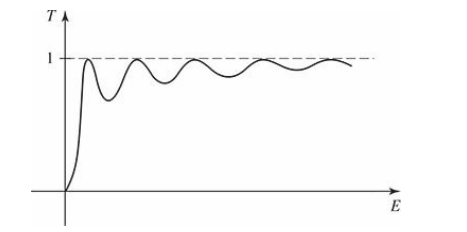
\includegraphics[scale=0.85]{RTeffect}
\end{center}
Here we consider a potential well described by the following:
\begin{align*}
V(x) = 
\begin{cases} 
0 & x<-a\\
-V_0 & -a\leq x\leq a\\
0 & x>a
\end{cases}
\end{align*} 
For the region $x<-a$, which we call the Region I, the wave function of a particle experiencing $V(x)$ is given by:
\begin{align}
\psi_I(x) = Ae^{ikx} + B e^{-ikx}
\end{align}
For the region $-a\leq x \leq a$, which we call the Region II, the wave function of a particle experiencing $V(x)$ is given by:
\begin{align}
\psi_{II}(x) = Ce^{ilx} + De^{-ilx}
\end{align}
For the region $x>a$, which we call the Region III, the wave function of a particle experiencing $V(x)$ is given by:
\begin{align}
\psi_{III}(x) = Fe^{ikx} + Ge^{-ikx}
\end{align}
Note further that the particle in Region II is not a free particle, and the time independent Schrodinger's Equation for such particle is given by:
\begin{align*}
\left( - \frac{\hbar^2}{2m}\frac{d^2}{dx^2} -V_0 \right) \psi_{II} = E\psi_{II}
\end{align*}
from which we obtain an expression of $l$:
\begin{align*}
\frac{\hbar^2 l^2}{2m} = E+V_0
\end{align*}
To compute the coefficients $A,B,C,D,E,F,G$, we make use of the boundary conditions for the wavefunction. That is, we require the wavefunction and its derivative to be continuous at the boundaries $x= -a$ and $x=a$, which gives a total of $4$ boundary conditions. WLOG, we also assume that the particle is coming from the left, and hence we can assume that $G = 0$. Furthermore, the reflection coefficient of such system is given by:
\begin{align*}
R = \left| \frac{B}{A}\right|^2
\end{align*}
and the transmission coefficient of the system is given by:
\begin{align*}
T = \left| \frac{F}{A}\right|^2
\end{align*}
where we also require $T + R = 1$. Solving the system we obtain:
\begin{align*}
\frac{1}{T} = 1 + \frac{V_0^2}{4(E ( E+V_0)}\sin^2\left(\frac{2a}{\hbar}\sqrt{2m(E+V_0)}\right)
\end{align*}
from which we observe that, $1/T = 1$ whenever the following holds:
\begin{align}
\frac{2a}{\hbar}\sqrt{2m(E+V_0)} = 2al = n\pi \qquad\qquad \text{for some }n\in \Z
\end{align}
Rearranging we obtain the energy for which the transmission $T$ peaks:
\begin{align*}
E_n = \frac{\pi^2 n^2 \hbar^2}{8 ma^2}- V_0
\end{align*}
From the condition (5.18), we see that (5.16) satisfies $\psi_{II}(\pm a) = \text{constant}$, connecting the wavefunction $\psi_I$ and $\psi_{III}$ in Region I and III. That is the particle travels through Region II as if it does not see Region II when $T$ peaks at $1$, that is (5.18) is satisfied.\\


Next we consider a simpler step potential given by the following:
\begin{align*}
V(x) = \begin{cases}
V_0 & x>0\\
0 & x\leq 0
\end{cases}
\end{align*}
There is no bound state under this potential, all states are scattering states and can escape to infinity.\\

\textit{Classically}, if the incoming particle have $0<E<V_0$, the particle cannot exit in the region $x>0$ as the particle does not have enough energy to go through the potential step at $x =0$. Also \textit{classically}, if $E>V_0$, the particle can always goes into the region $x>0$, as the particle has enough energy to go through the potential step at $x=0$.\\

\textit{Quantum mechanically}, if the incoming particle have $0<E<V_0$, solving the system gives an exponentially damped wavefunction for the existence of particle in the $x>0$ region, and a sinusoidal wavefunction for the existence of particle in the $x<0$ region. That is, for $0<E<V_0$, the particle is discouraged to go into the region $x>0$, but it is not impossible. For the case where $E>V_0$, \textit{quantum mechanically}, solving the system yields both sinusoidal wavefunctions in $x<0$ and $x>0$ regions, but the amplitude of the wavefunction in the $x<0$ region is slightly lower as one will find $R\neq 0$. These \textit{quantum mechanical} result differs significantly from the \textit{classical} results.\\


\newpage
Here we consider a stationary wavefunction that solves the time independent Schrodinger's Equation $\hat{H}\psi = E\psi$. We can define a probability current:
\begin{align*}
j = -i \psi^* \frac{\pd \psi}{\pd x} + i \frac{\pd \psi^*}{\pd x}\psi
\end{align*}
Here we will show that $j$ is independent on $x$:
\begin{align}
\frac{\pd j}{\pd x} = -i \psi^* \frac{\pd^2 \psi}{\pd x^2} + i \frac{\pd^2 \psi^2}{\pd x^2}\psi
\end{align}
Utilizing the time independent Schrodinger's Equation:
\begin{align*}
- \frac{\hbar^2}{2m}\frac{\pd^2 \psi}{\pd x^2} + V\psi = E\psi
\end{align*}
(5.19) then reads the following:
\begin{align*}
\frac{\pd j}{\pd x} = -i \psi^* \left( -\frac{2m}{\hbar^2}(E-V) \right) + i \left(-\frac{2m}{\hbar^2}(E-V)  \right)\psi = 0
\end{align*}
In fact, $T+R=1$ is \textit{not true} in general, but when one has $V(-\infty) = V(\infty)$, one can use $j$ to recover the conservation $T+R = 1$, that is, the actual quantity that is conserved is the flux described by $j$. 

\newpage
\section[Time-energy Uncertainty Principle]{\color{red}Time-energy Uncertainty Principle\color{black}}
For an operator $\hat{A}$ that becomes an observable:
\begin{align*}
\hat{A}\psi_n  = a_n \psi_n
\end{align*}
We can consider a general state:
\begin{align*}
\psi = \sum_n c_n \psi_n
\end{align*}
for which the probability of observing $a_n$ is given by $P_n = |c_n|^2$, and the standard deviation of the measurement of $\hat{A}$ is given by:
\begin{align*}
\sigma_A = \sqrt{\langle \hat{A}^2\rangle - \langle \hat{A}\rangle^2 }
\end{align*}
If we further has an operator $\hat{B}$ which does not commute with $\hat{A}$, that is $[\hat{A},\hat{B}] \neq 0$. Heisenberg's Uncertainty Principle states that we have: \footnote{The Generalized Heisenberg's Uncertainty Principle is derived in Physics 453 HW6, Problem 6.}
\begin{align*}
\sigma_A \sigma_B \geq \left|\frac{1}{2i}\langle [\hat{A},\hat{B}]\rangle\right|
\end{align*}
\example In the case where we have $\hat{A} = \hat{x}$, and $\hat{B} = \hat{p}$, we obtain $\sigma_{x}\sigma_p = \hbar/2$. \\

It is well-known the time-energy uncertainty $\Delta E\, \Delta t \geq \hbar/2$, but \textit{time} should not have a distribution. One way to proceed is by considering an operator $\hat{Q}$  whose average measurement is time dependent, from which one can deduce:
\begin{align*}
 \left| \frac{d\langle Q\rangle}{dt}\right|\,\Delta t = \sigma_Q
\end{align*}
Here we can write, for the average measurement of a state $\psi$:
\begin{align*}
\frac{d\langle Q\rangle}{dt} = \frac{d}{dt}\left( \langle \psi |\hat{Q}\psi \rangle\right) &= \left.\left\langle \frac{\pd \psi}{\pd t}\right| \hat{Q}\psi \right\rangle + \left\langle \psi \left| \hat{Q} \, \frac{\pd \psi}{\pd t}\right\rangle\right. + \left\langle \psi \left| \frac{\pd Q}{\pd t}\,\psi \right\rangle\right.\\
&= -\frac{1}{i\hbar}\left\langle\left. \hat{H}\psi\right| Q\psi \right\rangle +\frac{1}{i\hbar}\left\langle \psi \left| \hat{Q}\hat{H}\psi \right.\right\rangle + \left\langle \frac{\pd Q}{\pd t}\right\rangle\\
&= \frac{i}{\hbar}\left\langle \psi\left| [\hat{H},\hat{Q}]\psi \right.\right\rangle+ \left\langle \frac{\pd Q}{\pd t}\right\rangle\\
&= -\frac{2}{\hbar}\frac{1}{2i}\left\langle [\hat{H},\hat{Q}]\right\rangle
\end{align*}
where we have assumed that $\langle\pd Q/\pd t\rangle$ approaches zero, by the assumption of our theory that \textit{operator does not depend on time}. Taking the absolute value of both sides, we obtain:
\begin{align*}
\left| \frac{d\langle Q\rangle}{dt}\right| \leq \frac{2}{\hbar} \sigma_H \sigma_Q
\end{align*}
from which we obtain:
\begin{align*}
\Delta E \, \Delta t \geq \frac{\hbar}{2}
\end{align*}





























\end{document}